\documentclass[12pt, a4paper]{article}
\usepackage[utf8]{inputenc}

% === MARGINS ===
\usepackage[margin=0.75in]{geometry}

% === INLINE FONT SIZE ADJUSTMENT ===
\usepackage{anyfontsize}

% === DATE & TIME FORMATTING ===
\usepackage{datetime}

% === IMAGE ===
\usepackage{graphicx}
\graphicspath{{./img/}}

\usepackage{caption}
\usepackage{subcaption}
\usepackage{float}
\newcommand{\img}[3][]
{
  \begin{figure}[H]
    \centering
    \includegraphics[#1]{#2}
    \caption*{#3}
  \end{figure}
}
% Usage: \img[width=...]{<path_to_img>}{<caption>}

% === HEADER & FOOTER ===
\usepackage{fancyhdr}
% Header & Footer for all pages
\pagestyle{fancy}
\fancyhf{}
\lhead{Problem Identification}
\lfoot{Team United}
\rfoot{\thepage}

% === INDENTATION ===
\usepackage{indentfirst}

% === TABLE OF CONTENTS ===
% links
\usepackage{hyperref}
\hypersetup{
    colorlinks
}
\newcommand{\setlinkcolor}[1]{
  \hypersetup{
    citecolor=#1,
    urlcolor=#1,
    filecolor=#1,
    linkcolor=#1
  }
}

% === REFERENCE ===
\usepackage[utf8]{inputenc}
\usepackage[english]{babel}
\usepackage{csquotes,xpatch} % recommended
\usepackage{url}
% \usepackage{hyperref}

\usepackage[
    backend=biber,
    style=authoryear-ibid,
]{biblatex}
\addbibresource{ref.bib}

% === APPENDICES ===
\usepackage[toc, page]{appendix}

% === INCLUDE PAGES FROM OTHER PDF FILES ===
\usepackage{pdfpages}

% === LANDSCAPE PAGES ===
\usepackage{lscape}

% === ROTATING IMAGES ===
\usepackage{rotating}

% === BULLETS INSIDE TABULAR ===
\usepackage{booktabs}% http://ctan.org/pkg/booktabs
\newcommand{\tabitem}{~~\llap{\textbullet}~~}

% === ENUMERATE ===
\usepackage[shortlabels]{enumitem}
% Usage: \begin{enumerate}[a.] or [a)] or [(A)] etc.


\begin{document}

% ===== Cover Page =====
\thispagestyle{empty}
\vspace*{\fill}
\begin{center}
  \begin{figure}[h]
    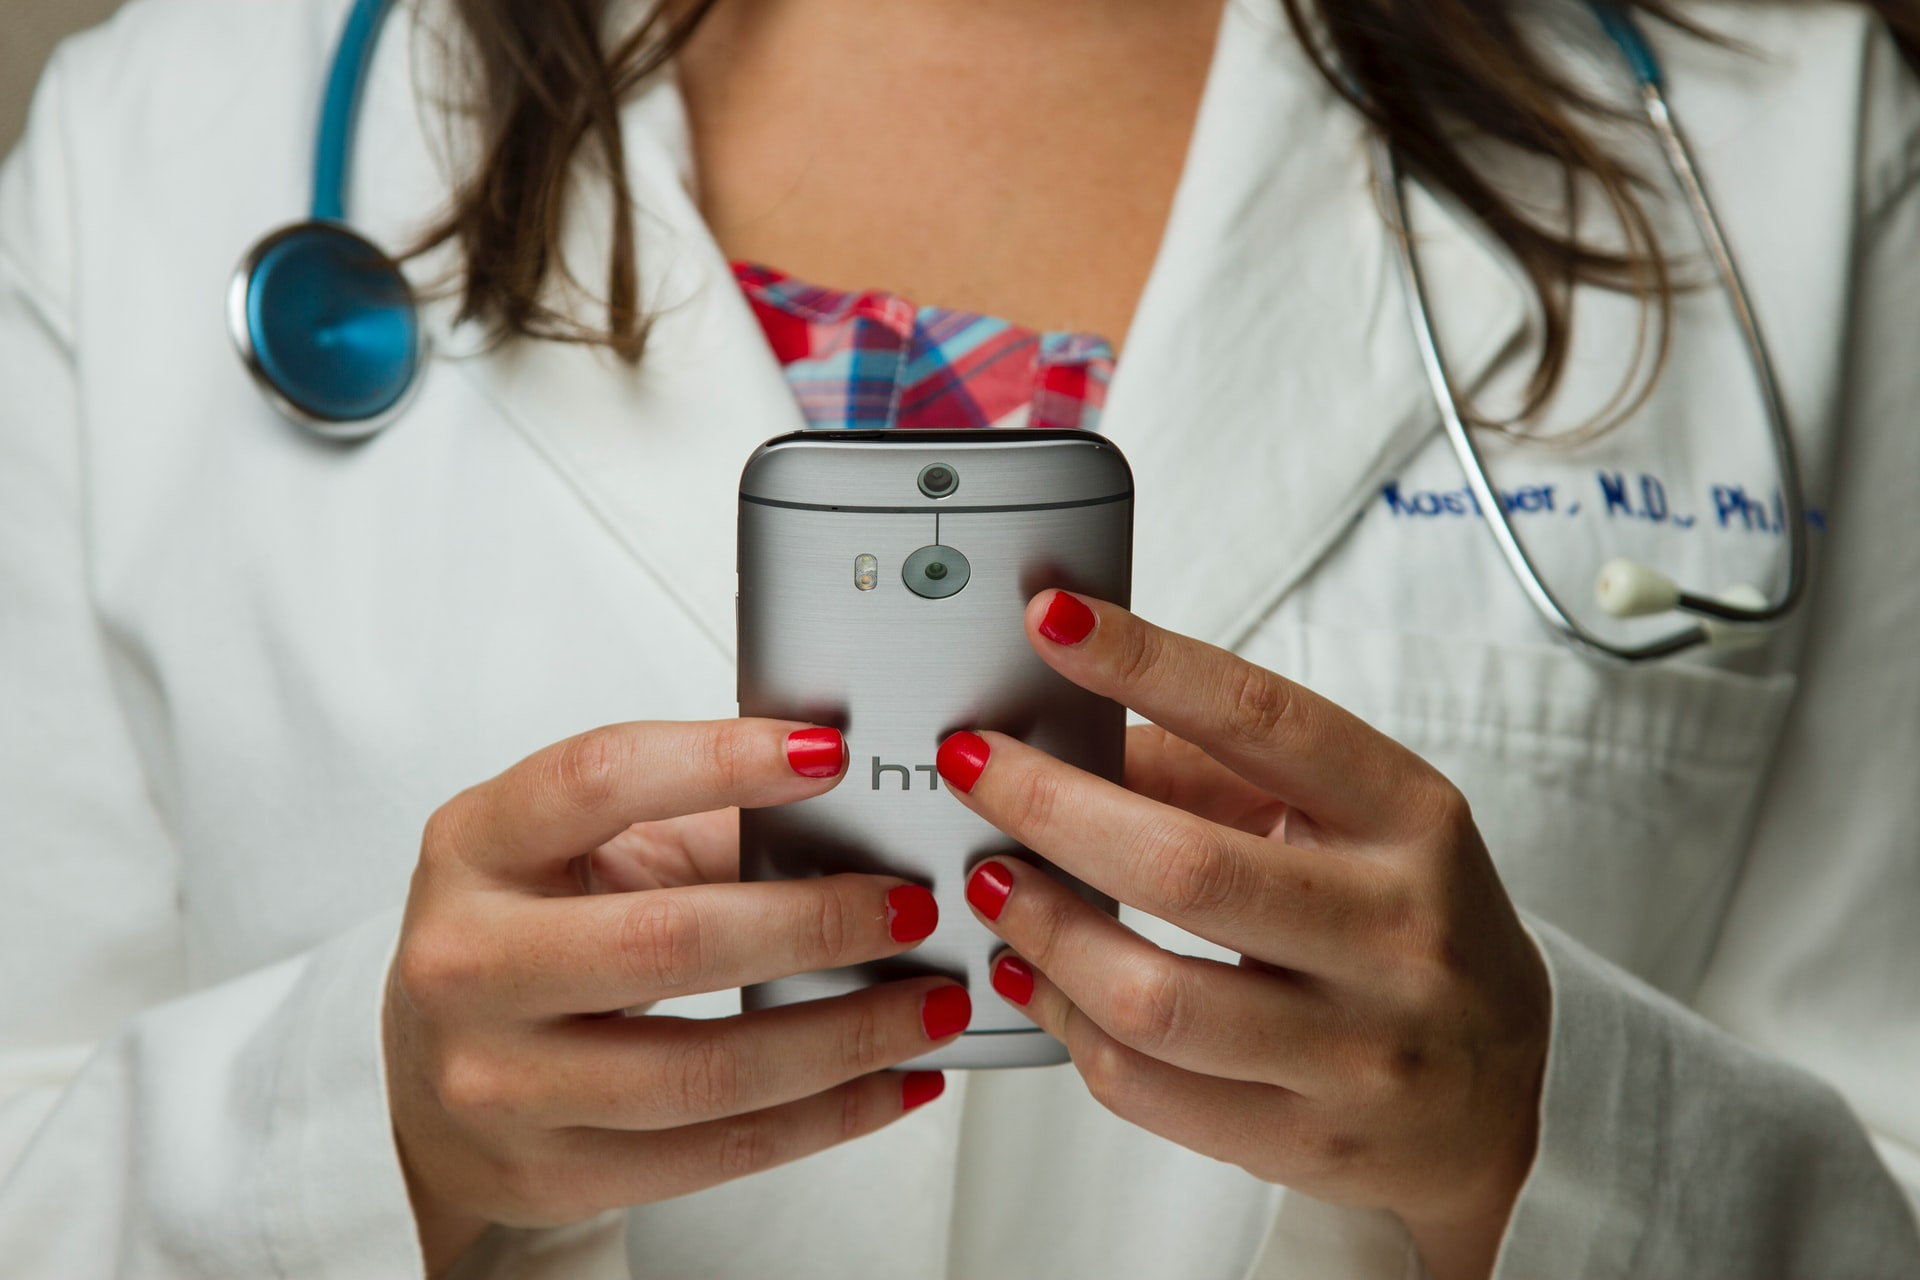
\includegraphics[scale=0.25]{cover-img.jpg}
    \centering
    {\footnotesize Photo by National Cancer Institute on Unsplash (https://unsplash.com/photos/cQ8FfVNvbew)}
  \end{figure}

  \vspace{2cm}

  \par {\huge Pandemic-countering Contact Tracing Application}
  \vspace{0.65cm}
  \par {\fontsize{40}{48}\selectfont Problem Identification Report}
  \vspace{0.5cm}
  \par {\LARGE Team United}
  \vspace{0.25cm}
  \par {\large  April 15, 2020}
\end{center}
\vspace*{\fill}
    \setlinkcolor{black}
% ===== Table of Contents =====
\newpage

% Header & footer stype for this page only
\fancypagestyle{toc}{
  \fancyhf{}
  \lfoot{Problem Identification, DECO3800 - Proposal}
  \rfoot{i}
}

\thispagestyle{toc}

\tableofcontents


    \setlinkcolor{blue}
\newpage

% Start page numbering from here
\clearpage
\setcounter{page}{1}

\begin{center}
  \par {\huge Pandemic-countering Contact Tracing Application}
  \vspace{0.25cm}
  \par {\LARGE Team United}
  \begin{center}
    \begin{tabular}{ |c|c| }
      \hline
      Full name & Student ID \\
      \hline
      Nguyen Thanh Hai Huynh & 46225696 \\
      Minh Nhat Nguyen       & 46225753 \\
      Khac Duy Nguyen        & 46225744 \\
      Kai Wen Chern          & 45632475 \\
      Minh Quan Nguyen       & 46225735 \\
      Diep Hung Vu           & 46225762 \\
      \hline
    \end{tabular}
  \end{center}
  \par {\LARGE Design Computing Studio 3 - Proposal}
  \vspace{0.25cm}
  \par {\Large April 15, 2020}
\end{center}


\section{Introduction}
  \par In this first iteration - Problem Identification - of the on-going assessment report of the course DECO3800 - Proposal, we direct our concentration towards the problem space of pandemic outbreak, namely COVID-19 as of the reality right now, and how a contact tracing application system can remarkably help flatten the curve of infection rate.
  \par Throughout the report, we will discuss multiple aspects of the issue, which have all been organized into concrete headings. Nevertheless, our current main focus is doing background research on the virus and any existing technology-aided countermeasures, checking what questions we still need to answer, and planning how we will answer them to progress further in this project.

\section{Overview}
  \subsection{Motivation}
    \par The current COVID-19 virus pandemic we are experiencing is critically dangerous not only because it causes pneumonia to the victims but it is also fully capable of dispersing from human hosts without them even know they have already been infected.
    \par Without proper population control measures, the curve of infection rate can rise steeply, eventually up to a point that may as well compromise the entire health care systems/resources we have got.
    \par Therefore, controlling the spread of the virus is a must if we do not want to reach the point of no going back in this global pandemic catastrophe. And the best measure we have got in our hands now is contact tracing.
  \subsection{The Project and Overall Aims}
    \par Developing a mobile application that can keep logs of who the user has met and where the user has been to so that in case someone is diagnosed positive with the virus, anyone who has been in close contact with this person is put under surveillance and any places this person has been to can be considered going into lockdown for disinfection.
    \par Possible technologies applied: Bluetooth signals, GPS services
    \par Overall Aims:
    \begin{itemize}
      \item Quickly track down individuals with a high chance of being infected and prevent further spreading of the virus
      \item Ensure that people receive the required care from health organizations in a timely manner as well as preserve privacy for the users of the application
      \item Being a channel for organizations with authority to issue important announcements and credible/factual information to the wider public
    \end{itemize}


\section{Background Research}
  \citetrackerfalse

  \subsection{What is COVID-19?}
    \par COVID-19 is part of a large family of Coronaviruses which cause respiratory infections. The virus first emerged in December 2019, Wuhan City, China \parencite{HealthGovAU}.
    \par These infections can range from just common cold to more life-threatening diseases such as Middle East Respiratory Syndrome (MERS) and Severe Acute Respiratory Syndrome (SARS) \parencite{Q&A_WHO}.
  
    \par How did COVID-19 come into existence? \parencite{CoronavirusOrigin}
      \begin{itemize}
        \item Evolutionary biologist Jemma Geoghegan of the University of Otago pointed out that the genome of SARS-CoV-2 - the virus which causes COVID-19 - closely resembles those of other viruses already existing in wild animals. 
        \par ``There is a virus in bats, as well as a virus in pangolins, that shares similarities with the new virus that has appeared in humans," said Dr Geoghegan.
        \item Veterinarian and environmental scientist Hume Field from the EcoHealth Alliance stated ``We don't need to manufacture this virus, it exists in nature as it is". 
        \par Dr. Field continued, ``From a scientific point of view, that argument that it's a manufactured virus has been totally discredited".
        \item Despite the fact that many early cases of COVID-19 were related to a live animal market in Wuhan City, we are still incapable of making the claim that this market was the place where the virus made the species barrier jump from some animal to human. 
        \par ``To be honest, I'm not sure if we'll ever know that because the wet market has now been cleared and been decontaminated," Dr Geoghegan said.
        \item As studies have shown that, in terms of genetics, there is a 96 percent similarity between SARS-CoV-2 and a bat coronavirus.
        \par And it is also recorded in the past that both SARS-CoV-1, the virus which caused the SARS outbreak in 2003, and MERS‐CoV, the virus that causes MERS, are found in bats. 
        \par Those facts led Dr. Geoghegan to a conclusion: ``It's likely that this new SARS virus has a similar route, ..."
        \item ``Human interactions with live animals make a host jump more likely to occur," Dr Geoghegan confirmed. And it is clear that the live animal markets are where this kind of interactions happen on a daily basis. 
        \par ``These locations can act as mixing pots, and you can have animals defecating, urinating, they're stressed maybe, you're bringing together the different species that may not be together," infectious disease ecologist David Hayman from Massey University said.
        \par ``And if hand hygiene and stuff like that isn't optimal, then this is where you have the opportunity for an infection to go from one species to another, and that includes humans."
        \par Dr. Field also added that live animal markets are the ideal scenario for host jumping of a virus to happen:
        ``You've got this mixing of species and this potential mixing of viruses in these animals that are under stress, sick and dying as they've gone from their wild environment to the market."
        \item ``If bats are the reservoir hosts of this coronavirus, it probably co-evolved with them over millions of years of their evolutionary history." Dr Geoghegan said.
        \par A recent research Dr. Field mentioned has also discovered that the existence of coronaviruses in bats was dated back to, if not thousands or millions of years, at least 10,000 years.
        \par ``These are very robust and sort of long-term evolutionary relationships of these viruses with these bats," the veterinarian proposed.
      \end{itemize}

  \subsection{How does COVID-19 behave and affect humans?}
    \begin{itemize}
      \item Symptoms: \parencite{HealthGovAU}
        \begin{itemize}
          \item fever
          \item coughing, a sore throat and fatique
          \item shortness of breath
        \end{itemize}
      \item Patients may gradually develop these mild symptoms: aches and pains, nasal congestion, runny nose, sore throat or diarrhea.
      \par Some people may not even know they are infected as they neither experience any previously mentioned symptoms nor feel unwell.
      \par Approximately 80\% of the infected can recover without any kinds of special treatment. Statistically, for every 6 people infected with COVID-19, one becomes seriously ill and develops difficulty breathing. People more probable to be stricken by the virus are the elderly and anyone with historic medical issues such as high blood pressure, cardiovascular diseases or diabetes \parencite{Q&A_WHO}.
      \item The interval of time starting from a person catching the virus until he/she begins to show symptoms is called the ``incubation period", which can range from 1-14 days but most commonly around five days \parencite{Q&A_WHO}.
      \item As suggested by studies and preliminary information on the COVID-19 virus, depending on environmental elements like surface type, temperature or humidity, a few hours or even several days is how long the virus can survive on surfaces \parencite{Q&A_WHO}.
      \item COVID-19 does not disperse in the air as the main way the virus transmits is through droplets, which are already too heavy thus will quickly land on some surfaces, an infected person produces when he/she coughs, sneezes, or speaks.
      \par Nevertheless, these droplets can still float in the air for as far as 1 metre away from the infected person. Therefore, apart from touching contaminated surfaces and then your eyes, nose or mouth later on before washing your hands, being in close contact (within 1 metre) with a person having COVID-19 may also get you infected by breathing in those droplets \parencite{Q&A_WHO}.
      \item For the time being, no vaccine or antiviral medicine has been confirmed 100\% effective in the prevention and treatment of COVID-19.
      \par Since antibiotics only work on bacterial infections, they prove ineffective against COVID-19, which is caused by a virus \parencite{Q&A_WHO}.
      \item Reinfection \parencite{Reinfection_abcnews} \parencite{Reinfection_independent}:
      \par Does your recovery from the virus mean you are safe from it? Many people question whether we can be infected a second time by COVID-19. One such example, in South Korea, there are 91 cases tested positive again after testing negative. Jeong Eun-kyeong, director of the Korea Centers for Disease Control and Prevention, said that it might be the virus that is reactivated not the patients being reinfected. Some cases that tested negative one day and positive another day during hospitalization. This is a complicated problem because if the result of tests is wrong, we might discharge patients who are still carrying the virus. Scientists and doctors are still working on the data from those cases to learn more about the behaviors and characteristics of this virus.
      \par According to a study in Shanghai, approximately one-third of the tested patients develop poor levels of antibodies. Lack of antibodies being produced also means a lack of immunity. There is an idea to use antibody testing to find out who is immune to the virus and who is not. However, Mary Carol Jennings, a physician and vaccine scientist, said “the logistics of making tests widely and fairly available are fraught, and we shouldn't pin our hopes to a single strategy.” Donald Trump,President of the USA, also said that he wanted everyone to be tested by this tool before the country operates normally again.
      \par Although coronaviruses have existed for a while and we have certain knowledge about them, scientists are still not sure about the immune response to this coronavirus. They need more time to do experiments on blood samples from cases around the world before going into a conclusion. ``COVID-19 has emerged so recently, we know very little about whether or not an initial infection 'teaches' the immune system how to protect against a future infection," explained Mary Carol Jennings.
    \end{itemize}
  
    \subsection{How does COVID-19 spread?}
      \par According to \textcite{Q&A_WHO}, all of the followings are possible trasnmission routes of COVID-19:
      \begin{itemize}
        \item This disease spreads from infected patients to others whom they have been in contact with even during the incubation period.
        \item The virus spreads through droplets from the nose or mouth of the infected person when he/she coughs, sneezes or exhales.
        \item People may be infected by breathing in droplets from the one that they are talking to and this is the main reason why social distancing is important. The safe distance between is about 1 meter away from the infected person.
        \item This coronavirus can last on surfaces and objects (namely tables, chairs, elevator buttons, etc.) for hours or up to days. Consequently, people can get infected by touching these objects which contain the virus and then touch their eyes, nose or lips.
        \item Although the rate of catching this virus from the one that has no symptoms is modest, people still need to be extremely careful when approaching someone. The reason is that at the initial stages of the disease, there are some patients who just show very mild symptoms like coughing and they do not notice that they may be infected until these symptoms become more severe.
        \item Despite the fact that the virus may exist in feces from the infected person, the proportion of spreading through this way is negligible. All you need to do is washing hands before meals and after using the toilet.
      \end{itemize}

    \subsection{Precaution and Prevention}
      \par To help suppress and possibly eradicate this new devastating virus COVID-19, \textcite{Q&A_WHO} encourages all individuals to practice the following hygiene/safety habits:
      \begin{itemize}
        \item Wash your hands after returning home and before entering your workplace or public places. You can clean your hands with hand sanitizer or with normal soap and water.
        \item Keep the distance about 1 meter from others in public to not only protect yourself but also the community.
        \item Minimize as much as possible touching your face, eyes and nose.
        \item Make sure that your family members or whoever living with you practice good hygiene. Remember to cover your mouth and nose whenever you cough or sneeze so that your droplets cannot land on public items.
        \item Please self-quarantine if you feel sick. If you experiencing symptoms like shortness of breath, fever or cough, contact your local health department and follow their instructions.
      \end{itemize}

    \subsection{Existing Pandemic-countering Measures/Technologies}
      \begin{itemize}
        \item How China slows down the virus \parencite{ChinasMeasure1} \parencite{ChinasMeasure2}:
        \par The Chinese government is very strict in monitoring their people in public places. There are CCTVs everywhere with face recognition technology integrated to find out who is not wearing a facemask or detect who has high hypothermia. Whenever people enter a building or workplace, they must declare their personal information, scan the QR code and write down their travel history in the last few days. A few residents said that they feared the surveillance would continue after the pandemic outbreak had been stopped. Every time they go out, they always feel like being stalked by somebody.
        \par One of the reasons that China has done so well in stopping the pandemic is mass quarantine. The government turns large places such as stadiums and hotels into quarantine centers to prevent the virus from spreading to the community. Moreover, many hospitals, which mainly focus on COVID19-infected patients, have been constructed. Many ways of penalty and reward have been proposed by the government to make sure that their people follow social distancing regulations. China virus tracking teams are surprisingly responsive despite dense population. They quickly isolate the infected patient as soon as possible and their friends, family members or roommates.

        \item BlueDot \parencite{BlueDotHome} \parencite{BlueDotCNBC}:
        \par BlueDot is a proprietary software-as-a-service designed to track, locate and conceptualize infectious disease spread. It warns health care, government, business, and public health clients about a summary of an abnormal epidemic disease that its Artificial Intelligence has identified and the hazards it may pose. Big data plays a pivotal role in crawling data from hundreds of thousands of sources, including statements from official public health organizations, digital media, global airline ticketing data, livestock health reports and population demographics by using natural language processing and machine learning. It’s capable of swiftly analyzing extensive information every 15 minutes, 24 hours a day.
        \par Moreover, not only is Blue Dot discovering epidemic disease as soon as possible, but it can also understand how diseases might disperse all over the world, and then identify the potential consequences it might lead to. Furthermore, by collecting global airline ticketing data, BlueDot was also able to precisely determine the places which would have the highest volume of travelers from Wuhan, including Bangkok, Hong Kong, Tokyo, Taipei, Phuket, Seoul, and Singapore. As a result, the top 11 cities of their list were considered to be first places to be infected with COVID-19.
        \par Blue Dot was founded by Kamran Khan - an epidemiologist and physician, who is self-described as an “accidental entrepreneur”. The severe acute respiratory syndrome (SARS) outbreak in 2003 deeply motivated him to start the project and find better solutions for infectious disease threats in the future.

        \item Contact Tracing:
        \begin{itemize}
          \item What is Contact Tracing?
          \par Against such a novel and highly-infectious virus like Covid-19, as we do not yet have the vaccine, contact tracing is one of the most effective weapons. According to the website of Queensland Health \parencite{QueenslandHealth}:
          \par ``Contact tracing is a process used to understand how an infectious disease is spreading in a community. Contact tracing has two purposes: to figure out who a sick person caught an illness from, and to find out who they’ve been in contact with while infectious.".

          \item Singapore's TraceTogether, Israel's TheShield and a contact tracing system Apple and Google are currently working on:
          \par Some mobile applications with similar purposes have been put into use in some countries, namely ``TheShield" in Israel \parencite{IsraelTheShield} and ``TraceTogether" \parencite{SingTraceTogether} in Singapore. For ``TheShield", the app takes location data of the user and compares that to the locations of confirmed cases to check if the user is at risk of being infected. If the app confirms that the user is indeed at risk, the user can choose to report themselves to the health authorities after filling out a form. On the other hand, ``TraceTogether" uses a different approach to contact tracing. Rather than taking users' location data, the app utilizes a Bluetooth protocol that allows nearby phones in an area exchange signals with each other. Each phone will then remember other phones that it has exchanged signals with in the last 21 days. In addition, location data is not collected. Compared to the ``centralized" approach of ``TheShield", where all the data is stored in one database of the authorities, this ``decentralized" approach partly helps deal with the concern of user's privacy. Recently, a similar system to ``TraceTogether" has been proposed and under-developed by Apple and Google, where the location data will not be collected \parencite{AppleGoogleSys}. Having said that, this decentralized approach is also not perfect, especially when there have been evidences that Covid-19 does not only transmit through direct contact.

          \item MIT-developed app system that uses Bluetooth signals to aid contact tracing while preserving privacy \parencite{MIT_App}:
          \par “Find My \parencite{AppleFindMy} inspired this system. If my phone is lost, it can start broadcasting a Bluetooth signal that’s just a random number; it’s like being in the middle of the ocean and waving a light. If someone walks by with Bluetooth enabled, their phone doesn’t know anything about me; it will just tell Apple, ‘Hey, I saw this light,’” says Marc Zissman, the Associate Division Head at MIT Lincoln Laboratory and co-principal investigator of the project.
          \par The project is fundamentally expecting a smartphone to constantly transmit and keep a log of contingent signals using their system. Simultaneously, the smartphone traces chirps found from other devices and only logs vigorously considerable chirps for contact tracing — those radiated from within 1.83 meters and acquired for a precise period.
          \par Users would participate by downloading an application that supports this tool. After a COVID-19 diagnosis, those people would be given a QR code from a health agency. They can also transfer their log to the digital computer data storage by scanning this QR code. These logs could be scanned by everyone using the app through their smartphones. A warning could notify a phone owner of the estimated distance to an active case if the system found a match.
          \par “We’re not tracking location, not using GPS, not attaching your personal ID or phone number to any of these random numbers your phone is emitting,” says Daniel Weitzner, a principal research scientist in the MIT Computer Science and Artificial Intelligence Laboratory (CSAIL) and coprincipal investigator of this effort. “What we want is to enable everyone to participate in a shared process of seeing if you might have been in contact, without revealing, or forcing anyone to reveal, anything.”
          \par The selection is optional. Weitzner guarantees that the app would respect the civil and human rights to not use the tool. The best thing we can do is expect that the populace would cooperate with the project to slow down the COVID-19 outbreak. “We need a large percentage of the population to opt in for this system to really work. We care about every single Bluetooth device out there; it’s really critical to make this a whole ecosystem,” he said.  
        \end{itemize}

        \item Discussion on these measures/technologies:
        \begin{itemize}
          \item The mass population surveillance and forced quarantine approach taken by China and South Korea has proved highly effective in the situation of escalating infection rate witnessed in these two countries. Nevertheless, such pandemic control method fails to guarantee the rights of privacy for the Chinese and Korean citizens. Therefore, in nations where the state of viral infection is not too severe, alternative measures apart from that currently adopted by China and South Korea will be extensively more desirable.
          \item With respect to global pandemic prediction and monitoring, BlueDot is unquestionably the right tool for the job, but that is also as far as BlueDot can go. Where BlueDot succeeds in offering globally applicable pandemic-countering measures, it is, on the other hand, unable to effectively tackle the precise level of each and every individual. We can understand the incapability of BlueDot simply by just considering how massive the amount of data it is already processes at the moment to be able to achieve what it is doing, hence monitoring at individual level would introduce unimaginable loads of data to be handled. Moreover, directing personal data around the globe into the hand of a single organization definitely will make privacy concerns and ethical issues turn to an even worse path. That is why we are still calling for an accurate, individual-level control method and thus, contact tracing.
          \item Except for Israel's ``The Shield'' which requires users' location data to function, all other contact tracing mobile applications aforementioned such as ``TraceTogether'' by Singapore, the two systems developed by Google, Apple and MIT University and specifically to Australia - the ``COVIDSafe'' app \parencite{CovidSafe} - utilize only the Bluetooth communication technology and avoid the usage of GPS services or any kind of location data for that matter to assure users with privacy preservation. However, not only is COVID-19 known to transmit through close-quarter contacts, it can also survive on object surfaces for a long period of time, thus also infecting anyone who touches these surfaces. Not exploiting location data secures users' privacy to some extent yet at the cost of not being able to trace back highly infectious locations. Acknowledging this fact, our app aims to mitigate as many as possible the issues posed by or experienced in other approaches and exactly how we plan to do that will be presented shortly in next sections.
        \end{itemize}
      \end{itemize}

  \subsection{Privacy Concerns}
    \subsubsection{User Concern}
      \par High possibility of exposing the location shared by the user (IP Leak) to the any kind of data breaches that may disclose the information towards unauthorized outsiders. Most cases were happened with an unguarded architecture through connection (e.g. database) or information without implementing encryption technology \parencite{Ian1}. According to \textcite{Ian2}, various companies sell, use or analyse the data to cater their clients through studying consumer behaviour, which prompted users to share their location without providing disclosure of the privacy policy with clarity upon the data collected. A study shown that users are also worried of the location tracking could put their close ones at risk through studying their routine, making their closed ones vulnerable to crimes \parencite{Ian3}.

    \subsubsection{National Establishment}
      \par There is no universal data protection and privacy law to be complied by all the registered countries by far. It has been stated in \textcite{Ian4} that the respective country law is being complied whenever the data is transmitted between countries. Hence, the enaction of a universal privacy and protection law for all nations to comply would be a sophisticated process. However, large regional union (e.g. European Union) had established a regulation called General Data Protection Regulation (GDPR) which all EU countries are to pass this law on federal level for data collection and processing. This is a huge milestone for regional unions of countries with diplomatic collaborations to enact laws on a higher level for legislations.
      \par An online journal of European Union \parencite{Ian5} concludes that the GDPR regulation emphasize on the fundamental rights and freedoms of natural persons with regards to the processing and movement of data should be adhered to all legal rules set for the protection of natural persons.

    \subsubsection{Australian Law}
      \par Office of Australian Information Commissioner (OAIC) \parencite{Ian6} has provided how GDPR comply with Australian privacy laws. As Australia Privacy Act 1988 (APP) indicated that Section 14 of the Act namely Privacy Principles (IPPs) adopts various transparent information handling practices, Australia and EU countries are compliant with both regulations of GDPR and APP whenever information is made across borders (as mentioned above in National Establishment). As both regulations enacted have different governance structures and preservation upon human rights. I will list the notable differences in information handling practices between both regulations.

\begin{table}[H]
  \begin{tabular}{|p{5cm}|p{5cm}|p{5cm}|}
    \hline
                                  & GDPR                                                                                                                                                & APP                                                                                                                                                                     \\
    \hline
  Compliance                     & \begin{tabular}[c]{@{}p{5cm}@{}} \tabitem Enterprise that have an establishment in the EU\\ \tabitem Enterprise that offers goods or services outside EU\end{tabular} & \begin{tabular}[c]{@{}p{5cm}@{}}\tabitem Australian Government Agencies\\ \tabitem Private Sectors and NGO\\ \tabitem Health Service Providers\\ \tabitem Small Medium Enterprise (SME)\end{tabular} \\
  \hline
  Types of Regulated Information & \begin{tabular}[c]{@{}p{5cm}@{}}\tabitem Collection of specific personal data (e.g. name, location data)\\ \tabitem Web cookies, routine data\end{tabular}           & \tabitem Collection of non-specific personal data that is reasonably identifiable (e.g. social circle)                                                                        \\
    \hline
  Consent                        & \tabitem Freely given, specific and informed with clear indication of written demonstration                                                               & \tabitem Express consent in written demonstration or implied consent through non-verbal communication                                                                         \\
  \hline
  Data Breach Notifications      & \tabitem A 72-hour timeframe to notify involved individuals and relevant authorities                                                                      & \tabitem Notify OIAC as soon as possible \\
  \hline
  \end{tabular}
  \end{table}

      \par In short, GDPR only applied to entities on enterprise level while APP on federal level. Next, GDPR
      will regulates information which includes personal activity data while APP considers data that could
      can be identifiable upon individuals such as social circle and household relationships. Furthermore,
      GDPR and APP both provides express consent for collecting data however APP allows entities to
      collect data upon implied consent as well, which may be unwilling under certain circumstances.
      Moreover, GPDR will allows a timeframe to be given for the entities to notify involved stakeholders
      upon data breaches whereas APP needs to notify the government agencies in an urgent manner.
    
    \subsubsection{Possible Alternatives}
      \begin{enumerate}[a)]
        \item \textbf{Cryptography}
          \par Asymmetric encryption could be a good option in enhancing data security level. Taking the proposing pandemic tracking app as an example, all users will have a public key to encrypt information sent to the application. On the other hand, the government as the application owners should hold the private key to decrypt the information only. \textcite{Ian7} written about a rotation mechanism that Apple uses to change the public key of a feature randomly from time to time, which increase the difficulties for anyone to track the users through location services (e.g. GPS, Bluetooth, hotspot, etc.). Hence, cryptography could be a useful implication to further support data security.
        \item \textbf{Union Law}
          \par As digital users have greatly increased during the recent decades, more people are able to obtain digital devices, such as smartphone for various purposes. In addition, the user community is expanding on a large scale across the globe, data is inevitably channelling across borders and regions, which is necessary for countries to establish unions that can collaborate for handling and exchanging these information (e.g. United Nation). Following data protection and privacy law, it is crucial that a universal law could be listed on legislations for all countries to comply with, that creates a standard of legal rules to protect the fundamental rights of a natural person.
      \end{enumerate}

  \subsection{User Research}
  \begin{enumerate}[1.]
    \item \textbf{Surveys}
      \par Survey is a method of quantitative research. It is used as an approach for collecting a more structured and statistical data for general background study. The participants were from various age groups as there is no conditional user restrictions, the possible solution is to cater all age groups.  Thus, collected responses are used for further evaluation to create a solution for general users. Moreover, this is a crucial process to understand the requirements for system visualization during design planning. The survey was designed through Google Form and made available online. The responses are attached below in Appendix \ref{appendix:quantitative}.
      \par \textbf{Findings}
        \begin{figure}[H]
          \centering
          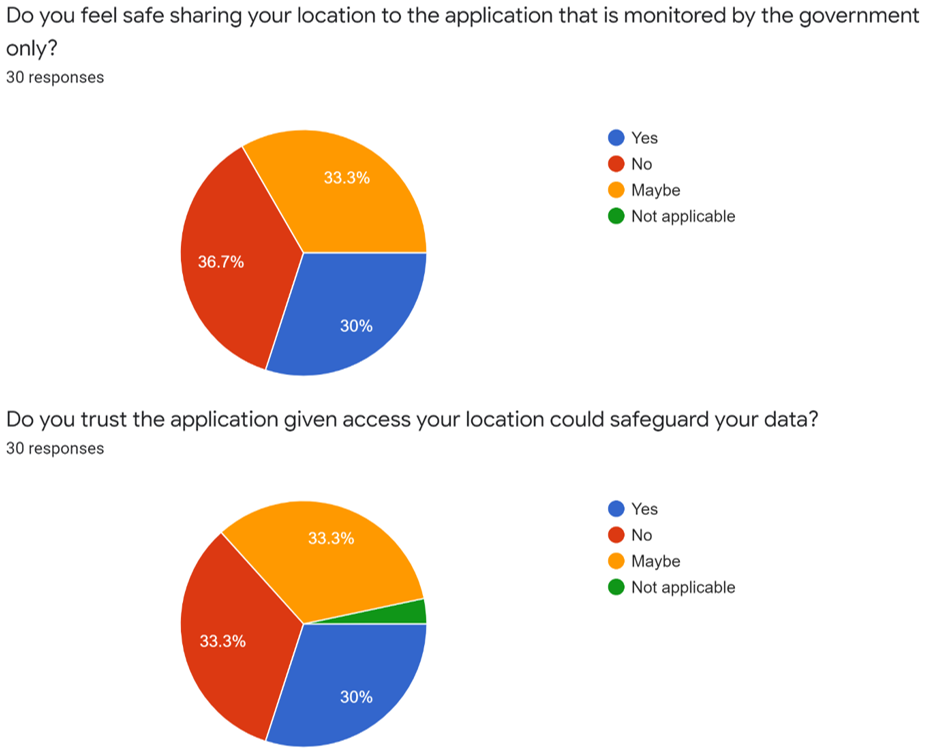
\includegraphics[width=14cm]{quantitative-01.png}
          \caption{}
          \label{fig:quantitative-01}
        \end{figure}
        \begin{figure}[H]
          \centering
          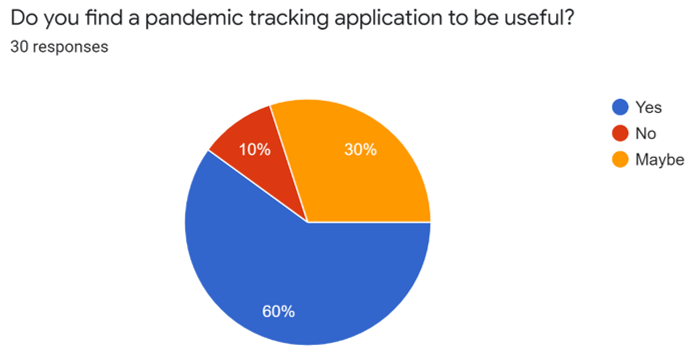
\includegraphics[width=12cm]{quantitative-02.png}
          \caption{}
          \label{fig:quantitative-02}
        \end{figure}
        \begin{figure}[H]
          \centering
          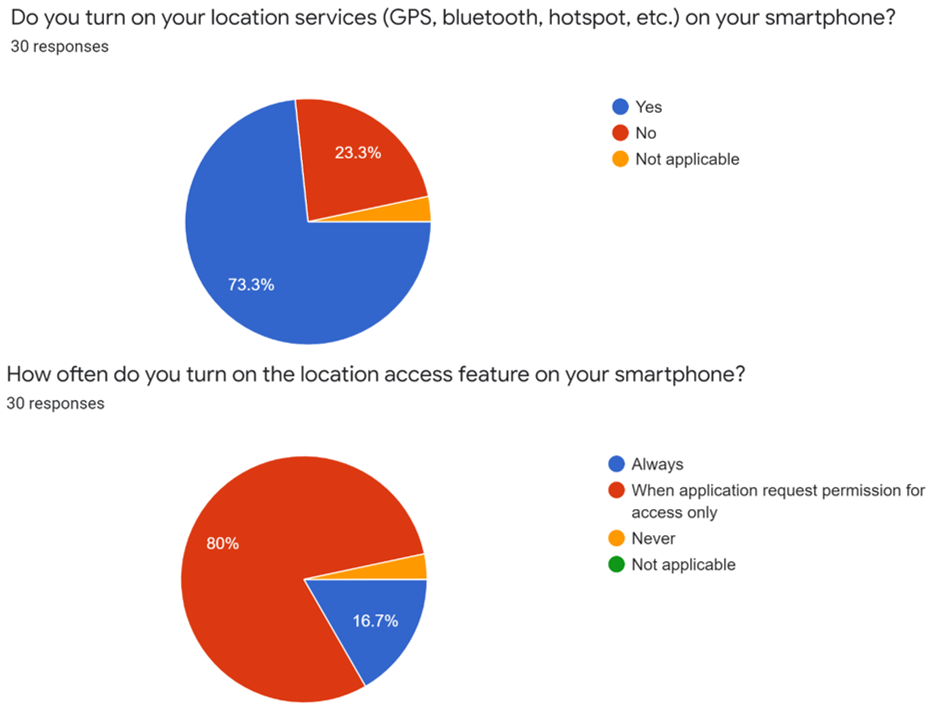
\includegraphics[width=14cm]{quantitative-03.png}
          \caption{}
          \label{fig:quantitative-03}
        \end{figure}

        \begin{itemize}
          \item Based on Figure \ref{fig:quantitative-01}, one-third of the respondents do not trust the data being protected regardless of it being a third-party or the government.
          \item Based on Figure \ref{fig:quantitative-02}, 60\% of the respondents thinks that a contact-tracing application would be useful.
          \item Based on Figure \ref{fig:quantitative-03}, approximately 73\% of the respondents turn on the location service feature which around 80\% gives location access only when the application request from the users.
        \end{itemize}
    \item \textbf{Interviews}
      \par Interview is a method of qualitative research. It is used as an approach for collecting descriptive opinions and views among different specific user categories. The interviewees were focused upon 3 different age groups consists of a primary school student, a retail worker, and a retired elderly that represents the age ranges of 0 to 17, 18 to 64, and above 65 respectively. The interview is composed of designed questions based on the evaluation from the survey, follow-up questions may also be included to gather more in-depth data. Thus, this helps to discover information based on their thinking, attitudes and even motivations. All interviewees have expressed consent to participate in this research study. The interviews were all conducted through online video call. The transcripts are attached below in Appendix \ref{appendix:qualitative}.
      \par \textbf{Findings}
        \begin{itemize}
          \item Minors do not think the application is necessary for them.
          \item Most adults are concern of the user privacy with location sharing.
          \item Includes accessibility features to accommodate elderly with disabilities.
        \end{itemize}
    \item \textbf{Insights}
      \begin{itemize}
        \item The number of application users could directly be influenced with the habit of users utilizing the location services or not, as it is necessary for the application to use the location services feature.
        \item Most participants do not trust the application to always collecting their location data.
        \item Most participants are doubtful of the government credibility in protecting their data. 
        \item Parental guidance and control could be a reason for minors not finding the application useful.
        \item Increasing accessibility features for accommodating user groups with disability could create a higher acceptance among the community.
        \item Proper digital privacy establishment is necessary for users to trust the application provider in handling their data.
      \end{itemize}
  \end{enumerate}

\subsection{What our app tries to achieve}
  \subsubsection{Contact Tracing}
  \par Same as many other existing COVID-19 contract tracing apps, our app will also utilize Bluetooth for close contact logging as this is the best technology we have got for the purpose. As for location logging, our team has considered the scenerio of still collecting location data using GPS services yet letting the users have the choice to opt out the functionality entiredly in case they have any privacy concerns. Based on the user research data displayed above, however, it was soon proven that the majority of users will feel reluctant, even resistive in some occasions, to the idea of live location tracking.
  \par To be able to still record location data and at the same time make the users feel somewhat comfortable with such function, our team has come up with a model that will be beneficial to all of the three important stakeholders - the government, the businesses and the users - as long as each of them agrees to take up certain responsibilities:
  \begin{itemize}
    \item What each stakeholder wants:
      \begin{itemize}
        \item The government: minimizing the number of COVID-19 cases as well as keeping the economy alive, hence complete lockdowns are not desirable.
        \item The businesses: staying open to make money.
        \item The users: being able to freely travel outside yet not risking being infected with COVID-19.
      \end{itemize}
    \item The solution:
      \begin{itemize}
        \item Avoid going into lockdown as much as possible. Consider it as the last resort only.
        \item The government enforces on businesses which wish to stay publicly open a law: businesses must log each and every customer who has visited their place. This can be done via QR codes given from the government to these businesses.
        \item Users must use our app to scan the QR codes of places they want to visit. Businesses have the right to ask and check if their customers have scanned the code. 
        \item As for places without closure like parks, squares, etc. the government can choose to close them up entirely.
      \end{itemize}
  \end{itemize}
  \par The following image summarizes our model:
  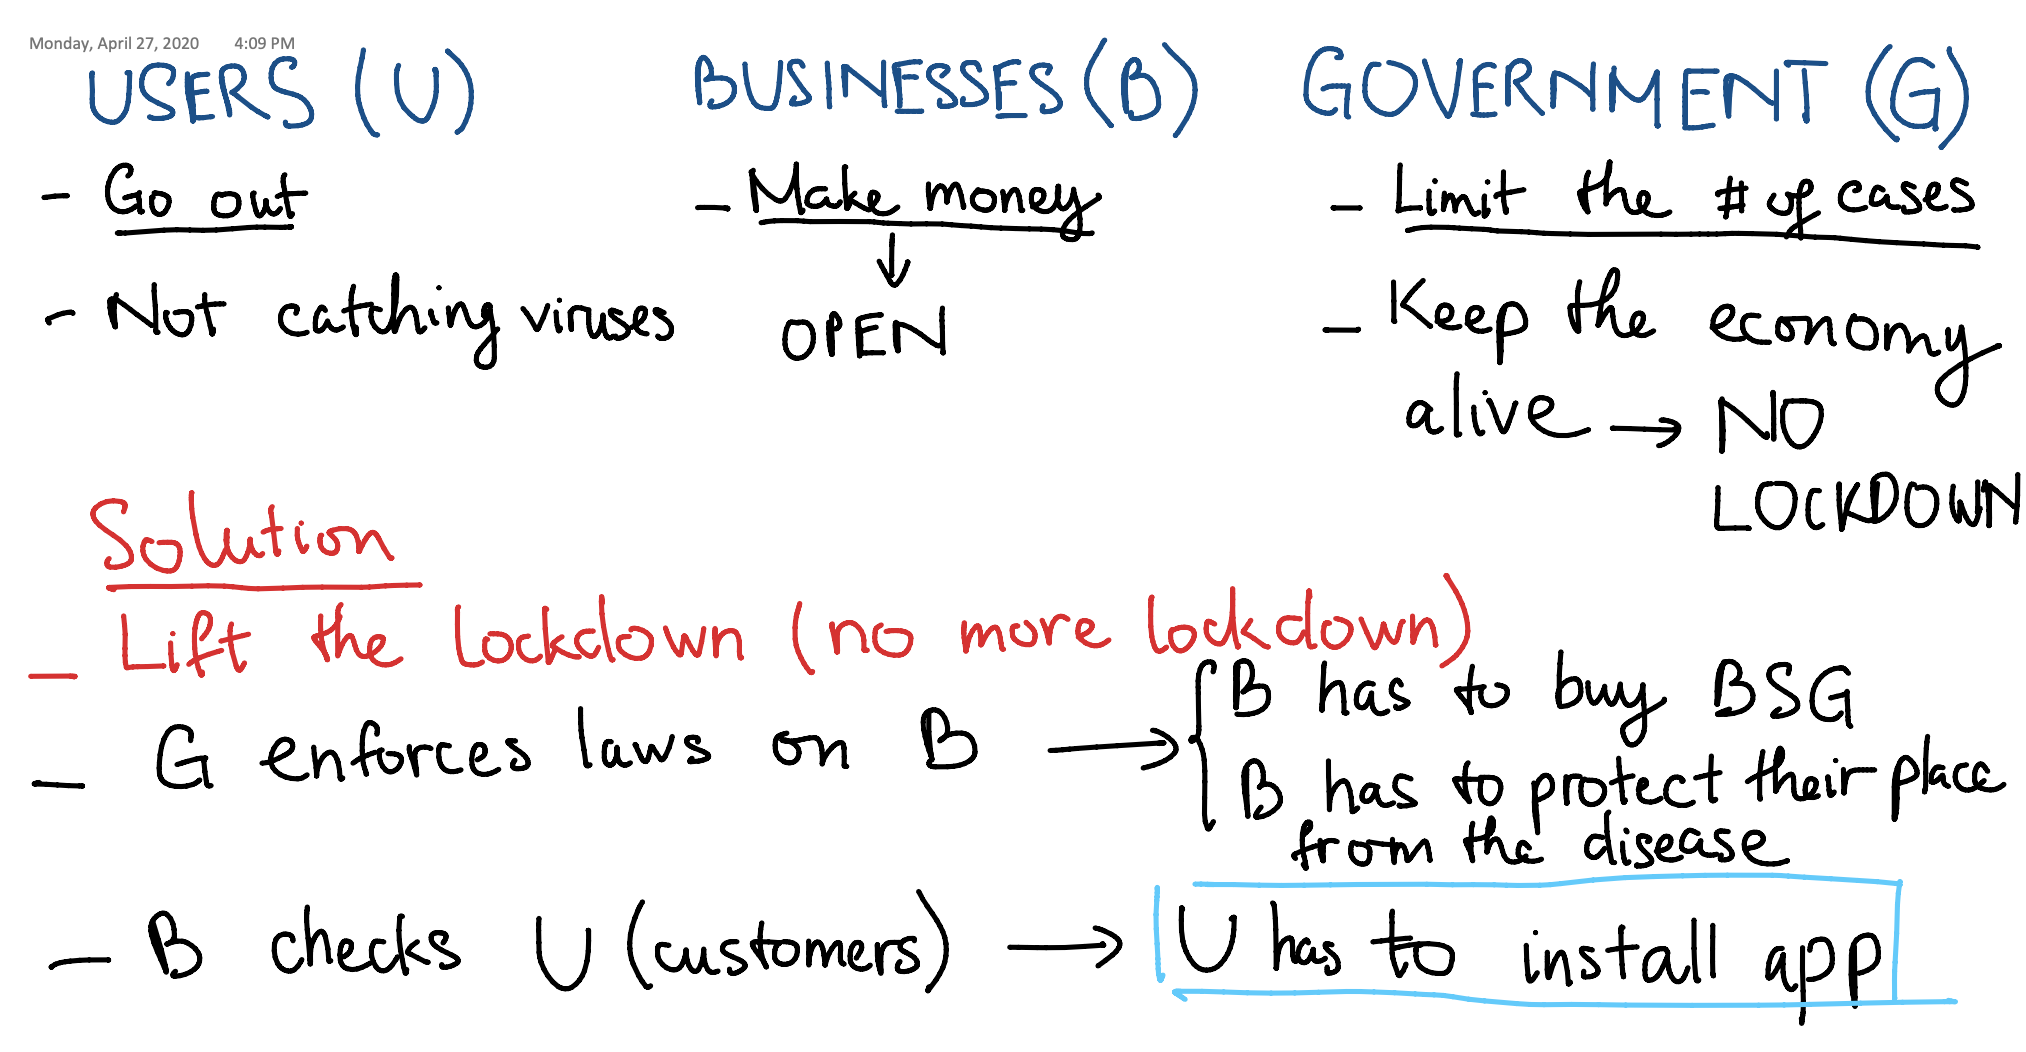
\includegraphics[scale=0.2]{solution-model}
  \par ``BSG'' stands for Bluetooth Signal Generator, which used to be our method of choice for location logging at business until it was found to be impractical to implement. Therefore, we have moved to QR codes as the replacement.

  \subsubsection{Support during lockdown}
  \par Our app, in what other apps have yet to do so, provides different kinds of support for its users throughout the quarantine period:
  \begin{itemize}
    \item The app can be an official channel for people to receive announcements about financial support from the government \parencite{Support5} or care packages from businesses \parencite{Support1}. Users can directly register for these support packages on the app without looking anywhere further.
    \item All emergency/support contacts are listed within the app in terms of which state you are living in \parencite{Support1} \parencite{Support2} \parencite{Support4}. Phone/Online health consultation and medicine prescription are also available. Users can request home-delivered medical supplies from local pharmacies \parencite{Support2}.
    \item The app recommends websites, applications, other online/digital medias which the users can utilize to: \parencite{Support3} \parencite{Support4}
      \begin{itemize}
        \item Keep fit through exercises. Eat and sleep healthily.
        \item Pick up a hobby/Learn new skills: Cooking, Playing musical instruments, Reading, Drawing, Photography, etc.
        \item Get mental advice/support and stay in touch with others.
      \end{itemize} 
  \end{itemize}

  \subsubsection{The technical aspect}
  \par As previously mentioned, our team has changed from Bluetooth Signal Generator (BSG) to QR codes for public places location logging. The reason for this decision was that we discovered it was technically impractical for the BSG to communicate with many devices at the same time. The way Bluetooth communication between devices works is that these devices need to form a connection, also known as pairing with each other, for stable data transmission. Therefore, the BSG would need to keep pairing and unpairing with each device in the area to send them the location code, which becomes near impossible for a large quantity of devices like hundreds or thousands.


\section{Stakeholders}
  \subsection{Users}
    \par It is obvious that this app is designed for everyone around the world. All you need is a smartphone or a wearable device to install the app. At the time when the pandemic seems to be out of control, this app is a considerable solution that helps users gain more understanding of their health conditions. It cannot be denied that when the scene is extremely dangerous, social distancing is one of the best solutions to prevent the virus from spreading. However, there are some situations that people must go outside such as grocery shopping or medical appointments \parencite{Stake1}. It is impossible to lock yourself inside your house 24/7. This app will help to track all other people that the user has been in contact with when they were outside. Although the number of people might be modest thanks to social distancing, prevention is still compulsory. Moreover, there are specific jobs that people cannot work from home. People may be working in public services, in retail, in vital parts of the manufacturing sector or for the governments \parencite{Stake2}. These paramount jobs cannot be converted instantly into homeworking. Therefore, there will still be several people heading out for works facing a high risk of infection. This app will support those people by storing the data of everyone they have met at the workplace or on the way to work.
  \subsection{Doctors/Nurses}
    \par Doctors and nurses probably benefit a lot from this app. The more we prevent the virus from spreading, the less the pressure on them. In countries which are facing the pandemic like Italy, doctors have to make heartbreaking decisions about who receives the treatment and who is abandoned \parencite{Stake3}. Furthermore, because of the sudden rise in the number of infected cases, there is not enough equipment for health workers \parencite{Stake4}. Consequently, many of them are risking their lives curing patients. Healthcare workers are influential in the war with pandemics and protecting them should be the number one priority. If they are infected, they must be isolated for at least 14 days, which will deplete the already exhausted workforce \parencite{Stake5}. By reducing the number of cases, doctors will be in contact with fewer infected patients. Finally, the situation of the pandemic is serious does not mean that we neglect patients with other sicknesses.
  \subsection{Governments/Health Departments/Health Organizations}
    \par It cannot be denied that governments play an important role in stopping the spread of pandemics. They are the frontline and their decisions highly influencing the fight against the epidemics. The governments have adopted some regulations like social distancing to protect and support their people. It is the governments’ responsibility to track the virus and put an end to it. With this app, they can easily find out who the infected patient has been in contact with instead of inquiring him/her. The results came out from investigating infected patients might be inaccurate due to the unstable health condition of them. Another problem that the governments and health departments are facing during the pandemic outbreak is the shortage of hospital beds. For instance, in the US, many hospitals have become overloaded \parencite{Stake6}. Based on overseas experience, about one-fifth of people infected with COVID-19 need hospital care and 5\% will need intensive care because of their critical health status \parencite{Stake3}. Therefore, if the coronavirus keeps spreading with the ongoing rate, the number of infected patients will exceed the number of available beds soon. In response, the governments have built more field hospitals which only cure COVID-19 patients. As proof, a dedicated coronavirus field hospital is being built in Canberra which could cost more than \$23 million \parencite{Stake7}. This application helps to reduce the number of infected cases also means that governments can save a lot of money.
    \par Our app is designed to track and store all the data of people whom users have been in contact during the plague. In other words, our application is mediated between governments and users. Governments and Health Department have access to the database so that they can select which users are most likely to be infected. After that, our application will be the means of communication for the government to connect with those users.
    \par This application also needs the cooperation of the Health Organization or Health Department to obtain all the information about the current pandemic (namely symptoms, how it spreads, how to protect yourself, etc.). With these data, the application can adapt and use the most effective tracking method.
  \subsection{Businesses}
    \par Not only a health concern, COVID-19 is seriously impacting business and the economy. It cannot be denied that this pandemic is affecting many aspects of the economy. According to data from the Australian Bureau of Statistics (ABS), approximately 90\% of businesses in Australia were expected to be impacted in the near future if the current situation continues \parencite{Stake2-1}. It can be said that the hospitality industry is the hardest hit. The severe crises that the hospitality industry is suffering from are worse than those of 9/11, SARS, and the financial crisis in 2008 \parencite{Stake2-2}. Many flights have been canceled, leading to a loss of aviation in every country. Restaurants and hotels are closed due to social distancing rules and the fact that no one dares to go out during the pandemic outbreak. There are some restaurants that are still open, but the government only allows them to serve takeaway food. This industry contains lots of family businesses like eateries, coffee shops, pubs, bistros, etc. Being a family business means that things will get even tougher as the demand falls and change in the supply chain \parencite{Stake2-2}. Some of them might totally shut down and wait for this virus to be contained so that they can continue their business.
    \par Apart from the hospitality industry, there are many other forms of the economy that are suffering no less. The number of unemployed people in the US have increased rapidly during the outbreak. In the first week of April, weekly total of new unemployment claims in this country reached nearly 7 million \parencite{Stake2-3}. Economists also warned that since the Great Depression in the 1930s, the world economy has never stagnated like it is now \parencite{Stake2-4}. Due to social distancing, people are asked to stay inside and only go out for necessary purposes. Consequently, the little demand for oil leads to a sharp drop in oil prices. For instance, oil prices in the US are negative for the first time the history \parencite{Stake2-3}. Coronavirus also changes how traditional commerce works. Letting people make transactions at banks is almost possible because according to social distancing restrictions, people must stay 1.5 meters away from others. Compliance with these rules while in the bank is impractical since banks are always crowded with people. Moreover, this virus can last on the surface of objects like bills, banknotes, or paper money. To tackle this issue, many banks have encouraged their customers to use digital banking instead of in-person banking or physical exchanges \parencite{Stake2-5}. Digital banking is feasible, but initially, it will face many difficulties such as training their staff to use digital tools. Furthermore, this virus is also the reason why many new companies afraid to enter the market.
    \par It is certainly true that when the disease outbreaks are severe, social distancing is the best method that we had to limit the interaction between people. But when the situation gets better, restrictions must be lifted so that businesses can open again. Although it is possible that the spread of this virus is under control, the government should not be too neglected because the possibility of reinfection of COVID-19 is still unknown. Therefore, our model is a reliable method to supervise the spread of this virus. Businesses can operate normally again if they agree to utilize our model and commit that they only serve customers who have the application installed on their digital device. By this approach, people will be more secure when they travel to places like restaurants, supermarkets, shopping malls, etc. and if the disease happens again, it will be easier for the government to find its origins.
    \subsection{Organizations}
    \par To achieve this model, there must be a way to encourage people to install it. If there is no way to attract people, it will be challenging to convince them to download the application. One is example is that the application named COVIDSafe, which is launched by the Australian government, only reached roughly 30\% of smartphone users age 14 and over after 18 days \parencite{Stake2-6}. It seems that one of the best solutions is to cooperate with organizations that are offering supports during the lockdown. There are lots of support packages out there for people during the pandemic outbreak:
      \begin{itemize}
        \item University of Technology Sydney offers support funds up to 15 million Australian Dollars to help students who are facing financial difficulties \parencite{Stake2-7}.
        \item Queensland government also has support packages for workers who have lost their job because of COVID-19 \parencite{Stake2-8}.
        \item Banks also make a move to help customers and businesses. To illustrate, BankSA has support for credit card and personal loan customers \parencite{Stake2-9}.
        \item One of the major telecom companies in Australia is Telstra offers supplementary data for users (register for 25GB of bonus data, unlimited data at home, unlimited call, etc.) \parencite{Stake2-10}.
      \end{itemize}
    \par By working with these organizations that have been mentioned above and more, it is more convincing for people to download the application. With this application installed on their digital devices, users will be given priority when registering for these support packages. Moreover, users can easily seek help via the application. There will be hotlines to health support departments, hotlines for people with disability who needs helps during pandemic outbreak and hotlines for those who are facing domestic violence and similar anxieties.




\section{Conceptual Model}
  \subsection{System Concept Statement}

    \subsubsection{One Sentence Problem Statement}
      \par Design and develop a mobile application that does pandemic contact tracing, guide the users on what to do next in case they have been exposed and provide further support during quarantine/lockdown.

    \subsubsection{High-level Description of the System}
      \par The system will:
      \begin{itemize}
        \item Conduct contact tracing:
        \begin{itemize}
          \item logging who the user has been in contact within the last 14 days
          \item logging the public places that the user has been to within the last 14 days in such a manner so that the user-business-government model is achieved
          \item notifying people who has come in close contact with a confirmed case so that they can voluntarily provide information about their current health status and contact the health department for testing
        \end{itemize}
        \item Guide the users step by step on what actions they should take once they have been notified of them possibly being exposed to a confirmed case.
        \item Supply the users with support services during quarantine/lockdown, including:
          \begin{itemize}
            \item Listing hotline numbers for health support
            \item Recommending resources that the users can utilize for health or recreational purposes
            \item Being an official channel for users to receive creditable information and register for care packages from organizations or the government.
          \end{itemize}
      \end{itemize}

    \subsubsection{Interaction Paradigms}
      \begin{itemize}
        \item Mobile: the application is installed on mobile devices
        \item Ubiquitous computing: Personal close contacts are logged automatically by the application. The user only needs to enable their Bluetooth services.
      \end{itemize}

    \subsubsection{Interaction Modes}
      \begin{itemize}
        \item \textbf{Exploring \& Browsing}:
          \begin{itemize}
            \item Notify the users if they have possibly been exposed to the virus through contacting with a confirmed case.
            \item Guide the users on what they should do so as to protect themselves, others and get tested if necessary.
            \item The user is recommended with mental and physical health improving or recreational resources to assist them throughout the quarantine/lockdown period.
          \end{itemize}
        \item \textbf{Instructing}:
          \begin{itemize}
            \item Enable Bluetooth services to activate the contact tracing mechanism
            \item Open the camera from within the application to scan location logging QR codes
            \item Link to websites for registering for care packages or financial support salaries
          \end{itemize}
        \item \textbf{Conversing}:
          \begin{itemize}
            \item The users can voluntarily choose to fill out a Q\&A form after they have been notified of the risk being exposed in order to provide the health departments with further information.
          \end{itemize}
      \end{itemize}
    
  \subsection{Design Guidelines}
    \subsubsection{UI/UX}
      \begin{itemize}
        \item The application should provide up-to-date and genuine information about the pandemic situation, while at the same time not causing unnecessary anxiety among the community.
        \item The simulation functionality needs to be fun and interactive in order to encourage people to learn about the pandemic and to make better decision in the pandemic situation.
      \end{itemize}

    \subsubsection{User Privacy}
      \begin{itemize}
        \item The system only collects minimal user data in order to function properly for the purpose of contact tracing.
        \item The system needs to be transparent about what data will be collected, and how data will be collected, stored, and used.
        \item The system has to allow user to decide and select what kind of data that they will share.
      \end{itemize}
    
    \subsubsection{Pervasiveness \& Scalability}
      \begin{itemize}
        \item Pervasiveness: The application should be fully functional on most mobile devices currently in use.
        \item Scalability: The system should be able to support millions (or even billions) of users.
      \end{itemize}
    
    \subsubsection{Information Security}
      \begin{itemize}
        \item The system have to strictly follow standard security guidelines of the industry.
        \item The system have to protect user from exposing their data to potential threats.
        \item The system will be open-sourced so that security issues can be detected as soon as possible.
      \end{itemize}

  \subsection{System Requirements}
    \subsubsection{Contact Tracing}
      \begin{itemize}
        \item The application utilizes only Bluetooth to conduct contact tracing in terms of personal encounters. As for location logging, to avoid involving any GPS services, we have decided to adopt QR codes scanning at specific public places as an alternative. The QR codes scanning implementation also makes sure that the government - business - user cooperation model is satified.
        \item Between Centralized and Decentralized contact tracing, our application complies with the Decentralized approach to maximize the amount of user privacy protection we can offer, thus, facilitating the users' trust in our system.
        \item Methods to guarantee users' privacy:
          \begin{itemize}
            \item Locally-generated Random Ephemeral User IDs: The ID attached with each user changes every two hours to ensure that no IDs can be exploited to trace back to a particular user.
            \item Voluntary Upload of Contact Tracing data: Although the application automatically notifies the users whether or not they have been exposed to the virus, it is entirely dependent on the users to take any actions that may follow, including uploading their contact tracing logging list up to the governmental centralized servers.
          \end{itemize}
        \item Only when a person is confirmed positive with the virus will he/she be given the permission to upload his/her contact tracing logging list up to the servers. The rationale behind this restriction is to ensure that no false positive cases are recorded into the system.
      \end{itemize}
    
      \subsubsection{User Guidance}
        \begin{itemize}
          \item In case the user has been notified that he/she is at risk of being infected with the virus:
            \begin{itemize}
              \item Ask the user to voluntarily fill out a Q\&A form consisting of multiple-choice and closed-ended questions that will assist the health organizations to extract further information from the user.
              \item Provide the user with step by step instructions on what should be done in order to protect himself/herself and the community.
              \item List country-specific emergency and health support hotlines in case the user may need them.
            \end{itemize}
        \end{itemize}
    
      \subsubsection{User Support}
        \begin{itemize}
          \item The official announcements from the government or any authorized organizations and departments delivered to the users should be timely, adequate and up-to-date.
          \item The application should offer a wide range of support packages that suit the needs of many different groups of users, for example, students, office employees, and construction workers.
          \item The application should only deliver crucial information such as virus spreading prevention techniques and useful resources that help the users stay healthy physically and mentally during quarantine/lockdown.
        \end{itemize}
    
  \subsection{Application workflow example}
    \begin{itemize}
      \item The user IDs are randomly generated locally on each user’s phone.
      \item When Alice and Bob come into close distance, the two mobile phones will exchange user IDs: Alice’s phone will save a copy of Bob’s ID and vice versa.
      \item Later, Bob is diagnosed and confirmed by the health department to have COVID-19.
      \item Bob is authorized by the health department to upload his “list” of close contact to the server. It is more like a “blackbox” than a list: no one can extract user IDs from it. When the app on Alice’s phone has downloaded the “blackbox” B from the server, it will do comparison locally like this: For each ID idi of Alice, the operation B(idi) will either output true if the idi is in the blackbox, or false if idi is not in the blackbox. If any ID of Alice is in the blackbox, the app will notify her.
    \end{itemize}      
    

\section{Questions/Areas of Investigation}
  \par The project raises many essential questions, including how such an app would address the issue of user privacy, whether the accuracy of collecting data for potential close contacts of such a system is precise, and whether it might be limited by environmental factors.

  \subsection{Privacy Concerns?}
    \par People from different countries have distinguishable opinions of privacy during the coronavirus pandemic. In China and South Korea, the authorities are publishing the movements of people before they were diagnosed with SARS-CoV-2 by tracking down their steps using GPS phone tracking \parencite{SingTraceTogether}. As a consequence, these approaches slow down the COVID – 19 outbreak since people are monitored and forced to quarantine themselves at home. Meanwhile, such a mandatory tool would raise serious concerns in many countries. People would argue that there are ethical factors with mass government surveillance that need to be considered. What if the populace cannot overcome concerns over human and civil rights? It should be clarified that how the app would manage personal details such as the user’s name, location, phone numbers, and by that way the governments still can easily identify the potentially infected people. Additionally, as establishing a national database may enable undesirable corporate, considerations for the security guarantee should be taken into account. Alternatively, using Bluetooth and QR code cloud-based systems for close contact logging could be the solution since these techniques are being used in reality to preserve users’ privacy. The app can give users the choice to opt-in or opt-out certain data that they allow or do not want the app to track. In this way, our app still provides services to users who opt-out and ensure users’ privacy safety.

  \subsection{How accurate are current technologies?}
    \par A GPS tracking surveillance system might seem like a good method, but the accuracy of data collection might be not exact. It is not easy as just identifying people have had direct exposure to patients or someone who potentially has SARS-CoV-2 since the reliability and precision of GPS technology remain in question. In China, some citizens report that even though they haven’t been in close contact with anyone with the virus, they find themselves stuck with “red code” that is applied to determine people are not allowed to move around freely or even return home \parencite{Questions2}. Another considerable concern is that there might be people who do not use smartphones or resist to use the app that will make serious challenges to the success of such a system. When it comes to the Bluetooth approach, our group faced questions about the technical aspect: Is it possible to make a wide-area-broadcasting Bluetooth signal generator? In our model, all businesses and public areas are required to have a mobile device with the same contact tracing app installed. Additionally, the range of the Bluetooth transmitter must be long enough to connect those specific devices to amplify the signal and cover the whole area so that if any user enters the area, their phone could log the code being broadcast in the area. Last but not least, our QR code approach also copes with difficulties such as controlling the crowd in public spaces (parks, beaches,...).
    
  \subsection{COVID-19 in the outer environment?}
    \par The approach of this project raises crucial questions about the virus’s behavior and environmental factors. One unclear feature is exactly how long SARS-Cov- 2 can live outside the host. Some researches on similar SARS-Cov-2-like viruses (such as Mers) suggested they can last on surfaces for as long as 9 days if these viruses are not disinfected. Some can live up to 28 days in low-temperature environments \parencite{Questions3}. These factors may lead to a situation: “You can sit within a few meters of someone and not be at risk. Meanwhile, it looks like you can come into contact with a train seat previously occupied by someone with the virus many hours earlier and be at risk,” said Assoc. Prof. Hannah Fry of University College London \parencite{Questions4}. Although the app actually cannot track all objects touched by confirmed cases and anyone having symptoms of the disease, the project should propose a suitable method to find the highest number of people with a high chance of being infected. When it comes to the final stage, multiple aspects of problems related to the virus's behavior remain unresolved. For the impact of these critical issues on the success of the project, the build team needs to investigate to find out what could we do to prevent environmental factors influencing the efficiency of our contact tracing application.

  \subsection{What features/services should the app offer?}
    \par To attract people to use, the app should offer features/services that other contact tracing apps do not have. User support during lockdown might be a good answer. Our group should figure out what people need during the quarantine in terms of finance, physical health, and mental health. The project also raised many essential questions: Do users agree to give more data if the app does benefit them more? Do users agree to install the app if the Bluetooth and QR code model is explained to them? For example, the TraceTogether app in Singapore had been installed by only 20\% of the total population \parencite{SingTraceTogether}. Meanwhile, such contact tracing apps require at least 40\% of the population to use its to make a high performance \parencite{Questions5}. If our group can assure users about what the app is doing, the success rate of this project will be enhanced. The final version of the prototype has proposed a complete solution of how the application would operate to offer users the most essential functionalities. As a comprehensive answer for what features should be integrated into a contact tracing application is subjective, the build team could also investigate to learn from the strengths and weaknesses of similar applications such as COVIDSafe and TraceTogether.

  \subsection{Conclusion}
    \par In sum, the project had an insight into important questions such as: What levels of privacy are people expected to sacrifice through using our app? What potential solution might be applied to improve the accuracy of data collection and enhance the effectiveness of the app?  How can we overcome limitations and challenges which are relative to environmental factors and the gaps in the knowledge about the virus behavior? Though our group successfully tackled most of the identified problems,  critical issues related to the environmental factors remain big  challenges that could prevent our contact tracing application from progressing properly. For that reason, the build team needs to carry out more researches into the behavior of the SARS-Cov-2virusas  well as to conduct more surveys, interviews to see if people agree to install our app and provide more of their data if doing so greatly benefits them more in COVID-19 prevention.



\section{Prototypes, Sketches, Studies}

  \subsection{Methodology}
  
    \subsubsection{Design Process Approach}
      \begin{figure}[H]
        \centering
        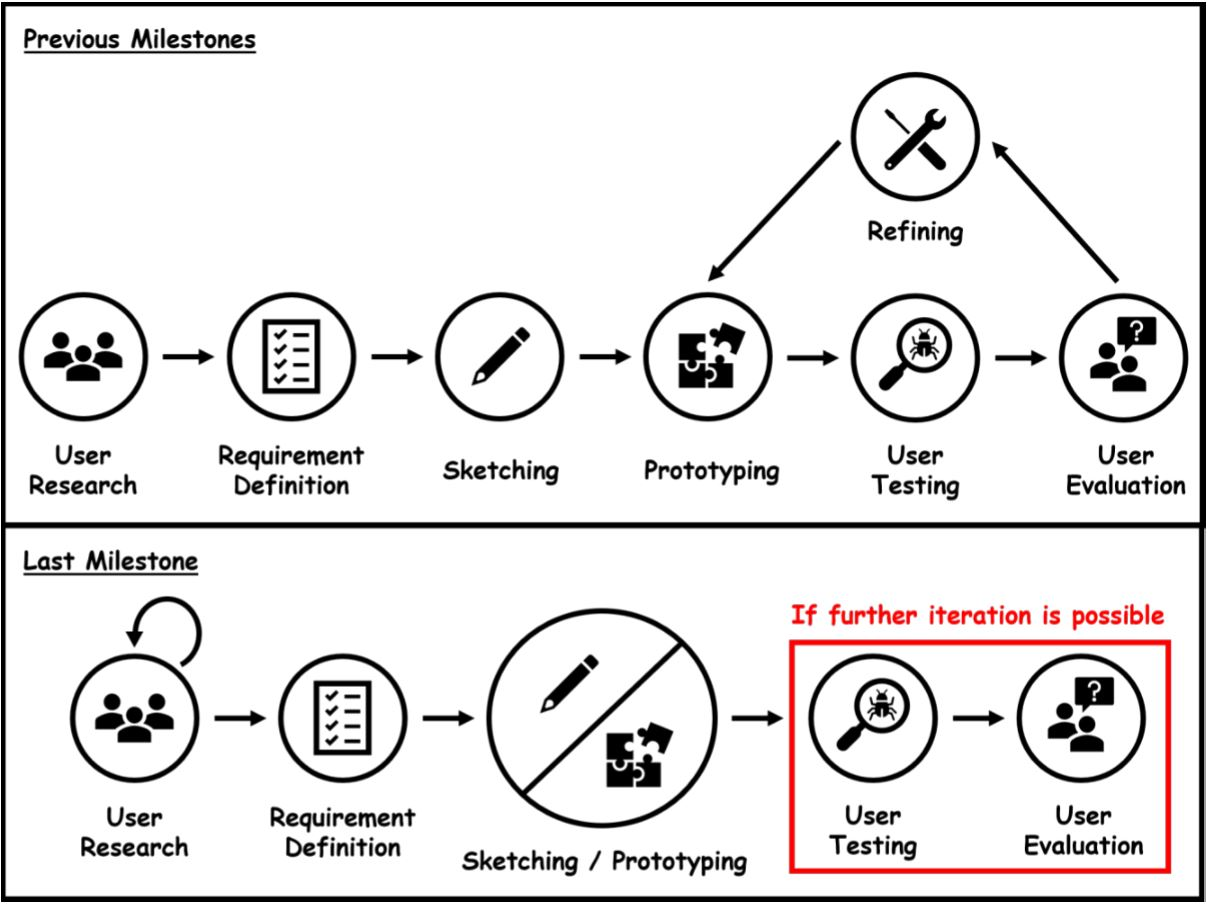
\includegraphics[width=\textwidth]{img/prototype/prototype-1.JPG}
        \caption{Prototype Design Approach}
        \label{fig:design-approach}
      \end{figure}
      \par \textbf{Summary}:
      \par As shown in figure \ref{fig:design-approach}, our approach for the previous milestones (iteration 1 and 2) were focusing
      more towards the implementation of designing and refining features based on how the users
      responded throughout the user testing session. With this approach, we had realized that refining the
      prototype specifications to display features that satisfy the users does not align with the initial
      concepts and goals we want to deliver as an application that deals with a pandemic outbreak situation.
      \par During the interim presentation with our peers and mentors, we received critiques of our proposed
      application does not have a core value to deliver to the stakeholders. After realizing what we are
      lacking, we revamp our design approach to specify our core values that the application should be
      delivered. With getting user inputs that are based on our application core values, we can illustrate a
      better prototype that satisfies the users with the prerequisite of fulfilling the core goals. As there are
      time constraints for the last milestone (iteration 3), we could only manage to proceed until the
      prototyping phase. Any user testing and evaluation can be done if there are any further iterations.

    \subsubsection{Terminology}
      \begin{itemize}
        \item \textbf{User Research}
          \par User research is to create assumptions for features that are necessary and crucial for the product user. It helps to create user personas for the target audience through representations of their demographics, habits, and behavior patterns. Various data collection methods are used to collect information in an iterative breadth-and-depth approach.
        \item \textbf{Requirement Definition}
          \par The information collected is analyzed to discover insights for involving quality features for the target
          audience. Hence, information can be compiled to create specific product requirements with proper
          documentation. The documentation would be the overview and detailed description of the methods
          used to create the prototype of our problem space by delivering our core values.
        \item \textbf{Sketching}
          \par Sketching helps to visualize features or the product contents to present how the illustrated
          components could help the users to achieve their goals upon using the product. It is to provide the
          best possible user experience with visual components and draft segments. It is encouraged to receive
          continuous feedback from users of the target audience for better visual input if possible. However,
          our last milestone (iteration 3) could only focus on creating the prototype by delivering our core
          values without further testing user input.
        \item \textbf{Prototyping}
          \par An interactive model of the product is created with integrating suitable visual components. The
          prototype could be developed with multiple iterations through collecting feedbacks during usability
          testing if possible. Despite that, we focused on creating a high-level prototype that deliver our core
          values on the last milestone (iteration 3) only due to time constraints.
        \item \textbf{User Testing}
          \par Usability testing is conducted with end-users of the target audience consisting of probing or think-
          aloud techniques and A/B testing for collecting user inputs. Various testing techniques will be
          explained below with more descriptive examples and statements. User testing is not being carried out
          in the last milestone (iteration 3). Any further iterations could perform user testing if possible.
        \item \textbf{User Evaluation}
          \par Product analytics could be made with analyzing and evaluate the user inputs upon the product for
          assessing the product potential. These inputs are studied for design and usability optimization. There
          is no evaluation as user testing is not carried out in the last milestone (iteration 3).
        \item \textbf{Refining}
          \par Prototype refinement made through the iterative and incremental process after user evaluation. This step
          is removed in the last milestone (iteration 3) as our team has created a goal to deliver the core values
          with an initial design for the prototype. Any further research could be carried out by another team.
      \end{itemize}

  \subsection{Research Study}
    \subsubsection{Data Collection Methods}
      \begin{enumerate}[a)]
        \item \textbf{Iteration 1}
          \begin{itemize}
            \item \textbf{Surveys}
              \par Survey is a method of quantitative research. It is used as an approach for collecting a more structured
              and statistical data for general background study. The participants were from various age groups as
              there is no conditional user restrictions, the possible solution is to cater all age groups. Thus, collected
              responses are used for further evaluation to create a solution for general users. Moreover, this is a
              crucial process to understand the requirements for system visualization during design planning. The
              survey was designed through Google Form and made available online. The responses are attached
              below in Appendix \ref{appendix:survey}.
              \par \textbf{Findings}
              \begin{itemize}
                \item Based on figure \ref{fig:findings-1}, approximate 33\% of the respondents do not trust the data being protected
                regardless of it being a third-party or the government.
                \item Based on figure \ref{fig:findings-2}, 60\% of the respondents thinks that a contact-tracing application would be useful.
                \item Based on figure \ref{fig:findings-3}, approximately 73\% of the respondents turn on the location service feature which
                around 80\% gives location access only when the application request from the users.
              \end{itemize}
              \begin{figure}[H]
                \centering
                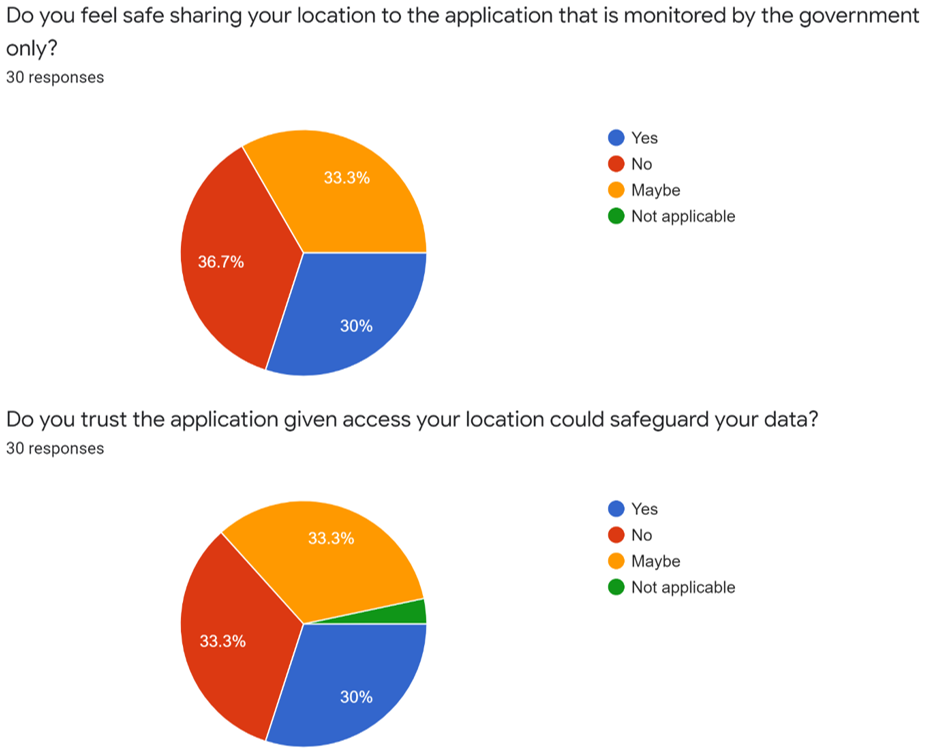
\includegraphics[width=\textwidth]{img/findings-1.png}
                \caption{Questions on Government Credibility to Safeguard Data}
                \label{fig:findings-1}
              \end{figure}
              \begin{figure}[H]
                \centering
                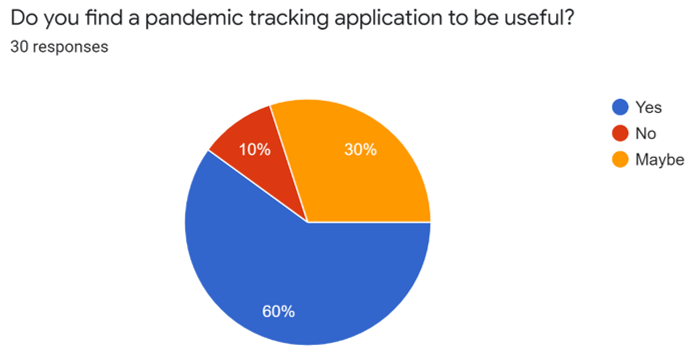
\includegraphics[width=14cm]{img/findings-2.png}
                \caption{Question on Usefulness of Pandemic Application}
                \label{fig:findings-2}
              \end{figure}
              \begin{figure}[H]
                \centering
                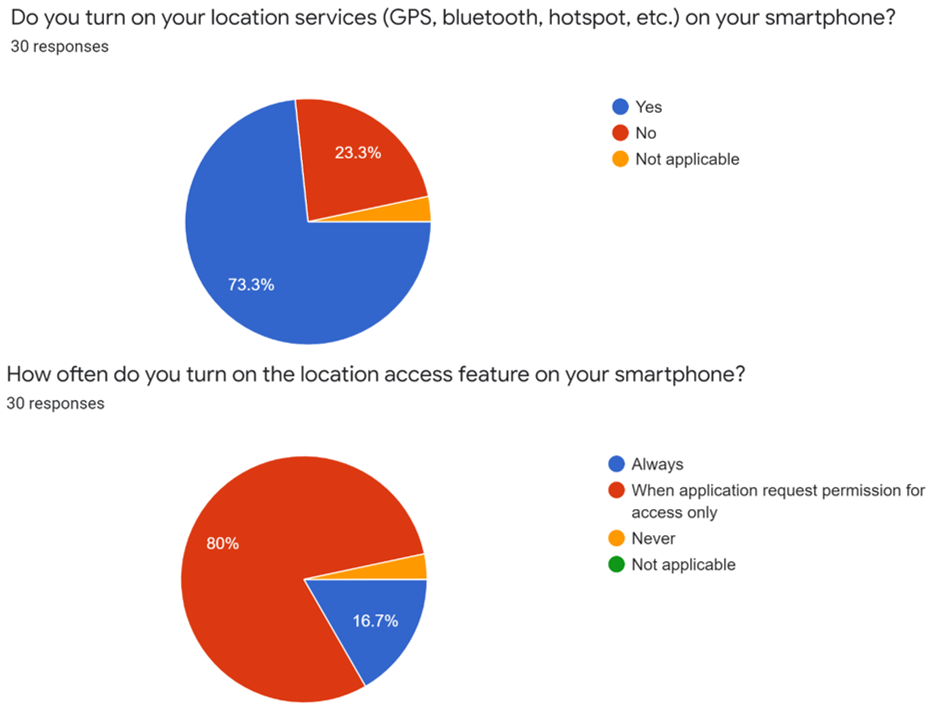
\includegraphics[width=\textwidth]{img/findings-3.png}
                \caption{Questions on User Usage on Mobile Location Access Feature}
                \label{fig:findings-3}
              \end{figure}

            \item \textbf{Interviews}
              \par Interview is a method of qualitative research. It is used as an approach for collecting descriptive
              opinions and views among specific users in different user categories. The list of interviewees was
              focused upon 3 different age groups consists of a primary school student, a young adult retail worker,
              and a retired elderly that represents the age ranges of 0 to 17, 18 to 64, and above 65 respectively.
              The interview is composed of designed questions based on the evaluation from the survey, follow-up
              questions may also be included to gather more in-depth data. Thus, this helps to discover information
              based on their thinking, attitudes, and even motivations. All interviewees have expressed consent to
              participate in this research study. The interviews were all conducted through online video calls. The
              transcripts are attached below in Appendix \ref{appendix:interview}
              \par \textbf{Findings}
                \begin{itemize}
                  \item Minors do not think the application is necessary for them.
                  \item Most adults are concerned with an application using location sharing.
                  \item Accessibility features implementation is a concern for the elderly community that includes disabled individuals.
                \end{itemize}
            \item \textbf{Insights}
              \begin{itemize}
                \item The number of application users could directly be influenced by the habit of users utilizing the location services or not, as it is necessary for the application to use the location services feature.
                \item Most participants do not trust any application that always collects their location data.
                \item Most participants are doubtful of the government's credibility in protecting their data.
                \item Parental guidance and control could be a reason for minors not finding the application useful.
                \item Increasing accessibility features for accommodating user groups with disability could create a higher acceptance among the elderly or disable community.
                \item Proper digital privacy establishment is necessary for users to trust the application provider in handling their data.
              \end{itemize}
          \end{itemize}
        \item \textbf{Iteration 2}
          \begin{figure}[H]
            \centering
            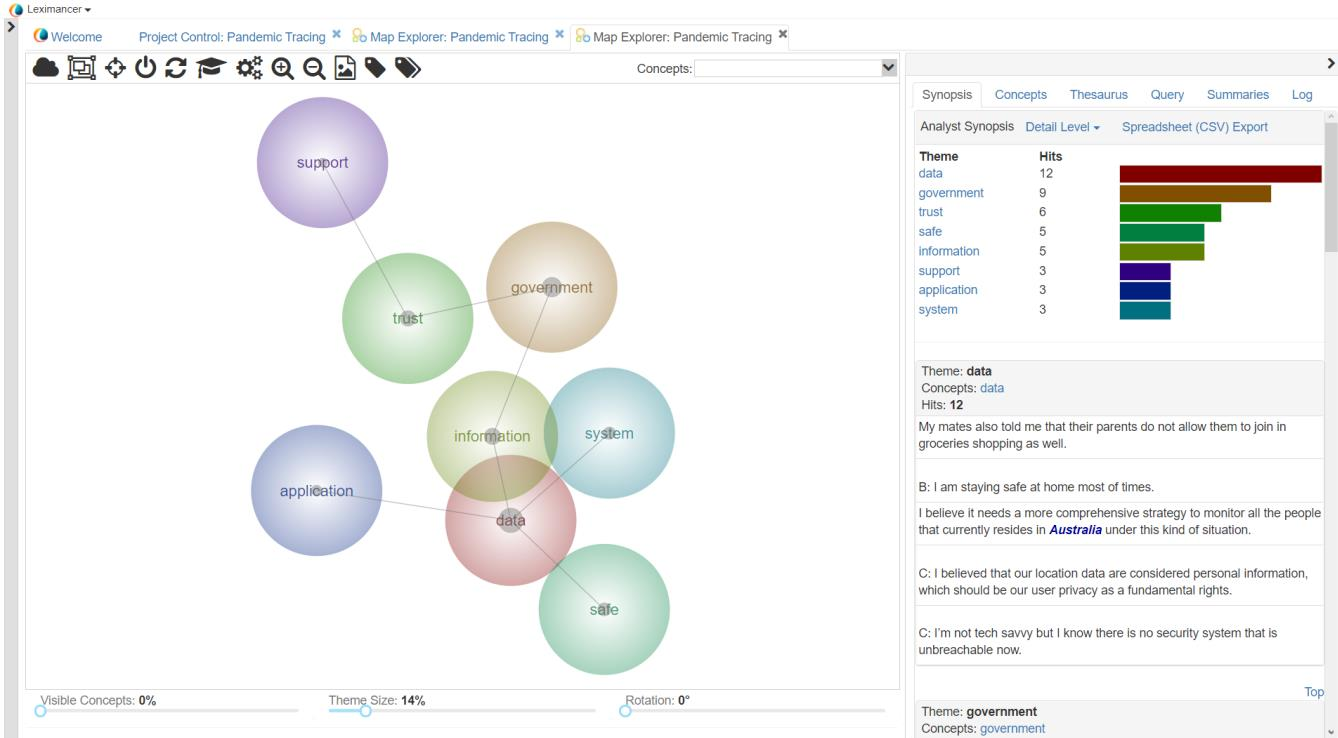
\includegraphics[width=\textwidth]{img/prototype/lexi.png}
            \caption{Text Clustering Analysis from Iteration 1 Interviews}
            \label{fig:findings-2}
          \end{figure}
          \begin{itemize}
            \item \textbf{Additional analysis}
              \par During Iteration 2, a text clustering was performed for the interview transcript generated during the previous milestone (Iteration 1). Text clustering is an application of cluster analysis for textual documents. It allows grouping for a different set of unlabelled words with similarity within the same cluster. Hence, this approach could further find insights from keywords mentioned from the interviews to further provide guidance for better decision making and define our project goals.
              \par Our approach to using text clustering includes the reasoning of lacking at least a core value for our product that should deliver to the target audience. With using this approach, we can identify some keywords mentioned many times such as ``support and ``trust" along with the previous survey insights generated from the previous milestone (Iteration 1) and further consolidate it to create our goals that identify the core values we want to deliver to the stakeholders as a pandemic tracking application.
          \end{itemize}
        \item \textbf{Iteration 3}
          \begin{itemize}
            \item \textbf{Surveys}
              \par As our team also realized how important data privacy should be considered during surveys while
              collecting data, all the involved participant ID will be masked and anonymized. The survey question
              would be related to our core goals and values that our application would like to deliver. The
              participants were mostly from the same group of the previous milestones (iteration 1 and 2). The
              survey was designed through Qualtrics and made available online. The responses are attached below
              in Appendix \ref{appendix:iter3-survey}.
                \begin{figure}[H]
                  \centering
                  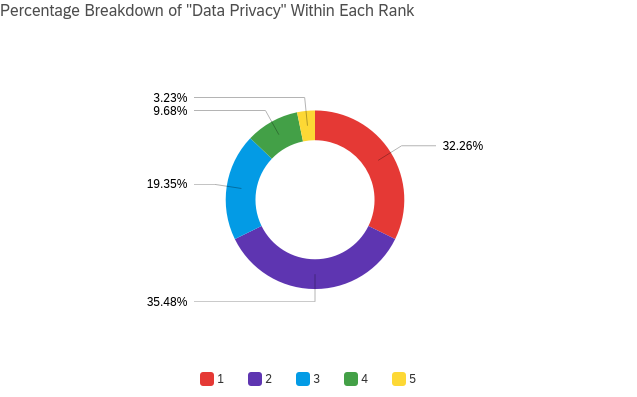
\includegraphics[width=\linewidth]{img/prototype/iter3-survey-findings-1.png}
                  \caption{Data Privacy Overall Ranking}
                  \label{fig:iter3-survey-findings-1}
                \end{figure}
                \begin{figure}[H]
                  \centering
                  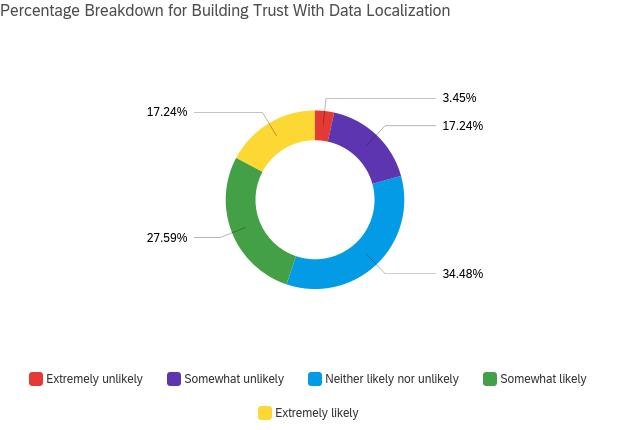
\includegraphics[width=\linewidth]{img/prototype/iter3-survey-findings-2.png}
                  \caption{Total Percentage Distribution of Building Trust with Data Localization}
                  \label{fig:iter3-survey-findings-2}
                \end{figure}
                \begin{figure}[H]
                  \centering
                  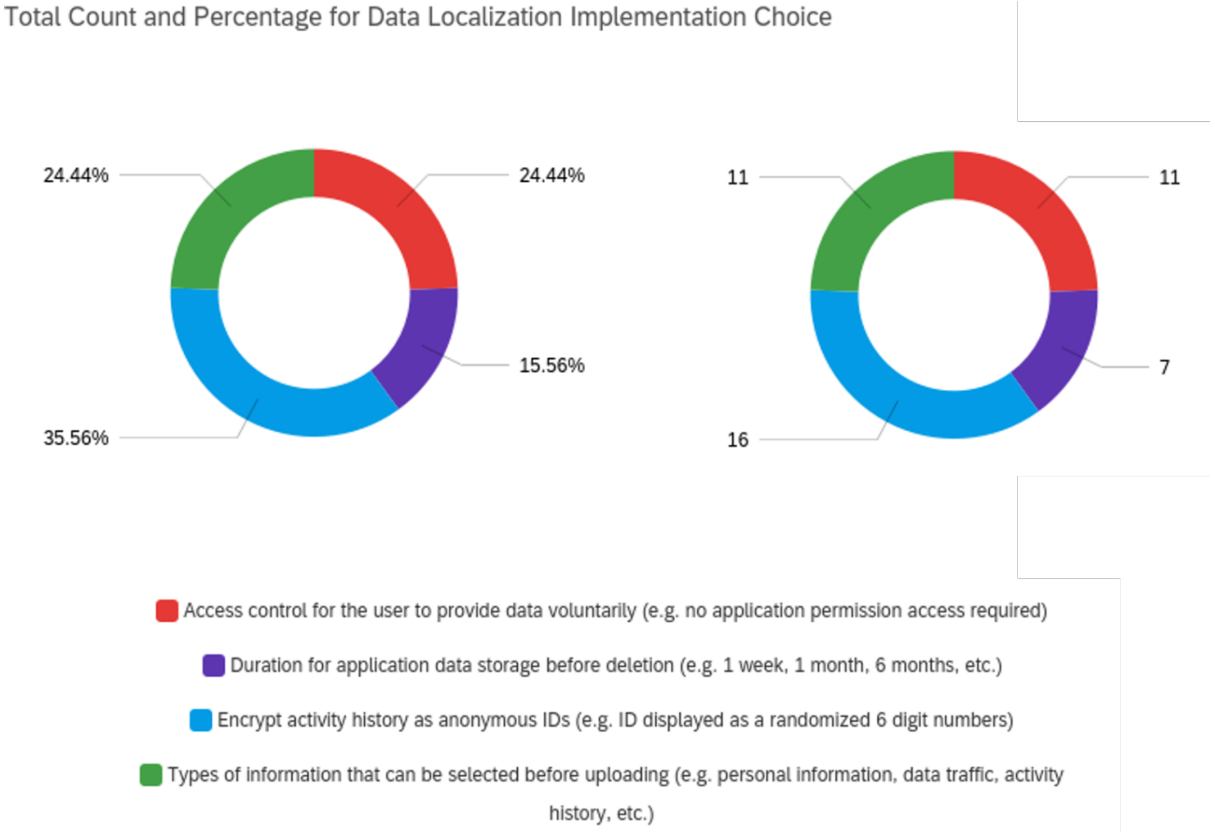
\includegraphics[width=\linewidth]{img/prototype/iter3-survey-findings-3.png}
                  \caption{Total Distribution of Count and Percentage for Data Localization Implementation}
                  \label{fig:iter3-survey-findings-3}
                \end{figure}
              \par \textbf{Findings}
              \begin{itemize}
                \item Based on figure \ref{fig:iter3-survey-findings-1}, respondents have rank data privacy as the top 1 and 2 priority in a mobile
                application which are approximately 32\% and 35\% respectively.
                \item Based on figure \ref{fig:iter3-survey-findings-2}, approximate 44\% of the respondents think that mobile application that implement
                data localization could build trust with the user.
                \item Based on figure \ref{fig:iter3-survey-findings-3}, the top 3 implementation choices chosen by the respondents include anonymous
                ID, access control for voluntary data upload and type of data upload which are 35\%, both 24\%
                respectively.
              \end{itemize}
              \par \textbf{Insights}
              \begin{itemize}
                \item Data privacy has proven to be an important factor for a mobile application throughout both survey
                sessions by similar respondent groups.
                \item Data localization could be a good concept to build trust with user for mobile application that
                requires data sharing.
                \item The choices chosen by the respondents for data localization implementation are closely aligned
                and related with our core values of the proposed application.
              \end{itemize}
          \end{itemize}
      \end{enumerate}

  \subsection{Sketches}
    \subsubsection{Simulation}
      \begin{enumerate}[a)]
        \item \textbf{Iteration 1}
          \begin{figure}[H]
            \centering
            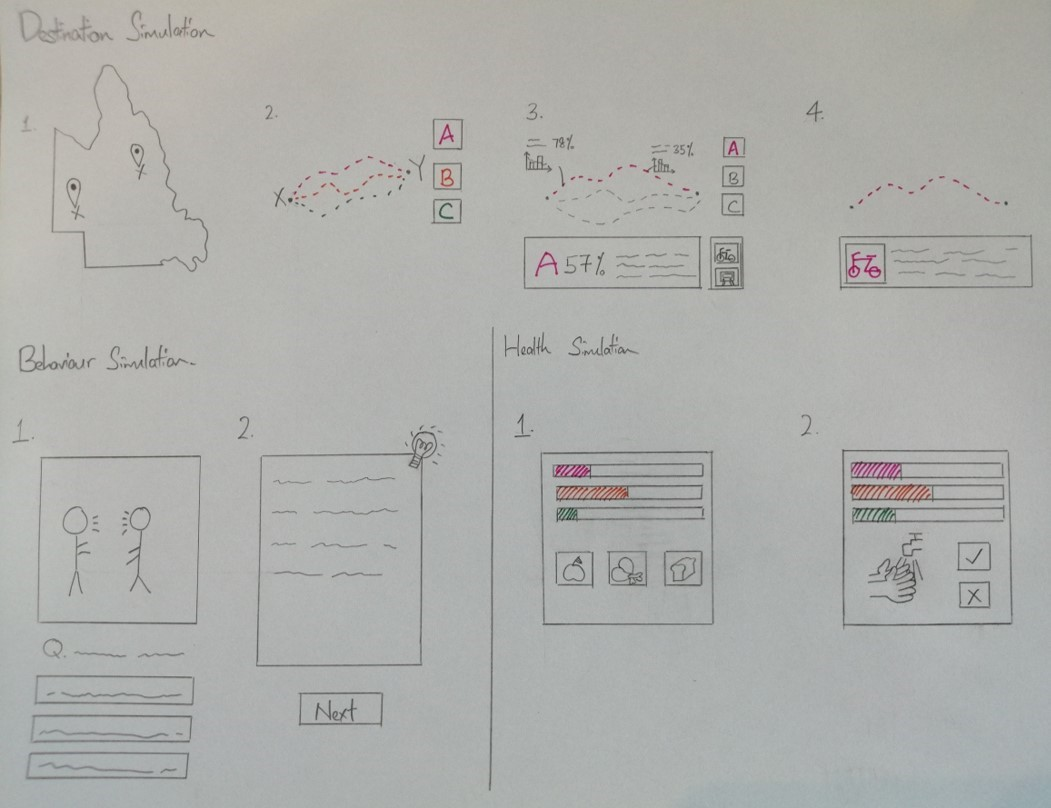
\includegraphics[width=\linewidth]{simulation.jpg}
            \caption{Simulation Sketches}
            \label{fig:simulation}
          \end{figure}
          \par Based on figure \ref{fig:simulation}, various simulations are considered during the first iteration. The sketches will be designed and showcased digitally to be interactable as a feature implementation for the proposed solution during the second iteration. The purpose of a simulation is to provide a learning opportunity for users. Furthermore, it promotes the application to be more educational through a human-computer interaction (HCI) design. Moreover, this will increase the user flow whenever the user interacts with the simulation, which creates possibility of more user scenarios in a simulated environment with real-life aspects during the pandemic outbreak. In addition, it provides a pleasant user experience when information is conveyed via gamification with audio and visual components. Hence, the information conveyed by the simulations to the user helps to deliver the values of the application. The simulation works with navigating the user through a journey that is projected with real-word aspects by embedding and implicit impressions which may turn into healthy habits and matured practices. In other words, it encourages habit and behavior changes when appropriate information is conveyed in an interactive manner that could be instilled into users under these special circumstances.
        \item \textbf{Iteration 2 and 3}
          \par There are no sketches created for the third iteration. As sketches are harder to illustrate the user
          scenario process of how data localization is implemented in our proposed solution. Our team decided
          to proceed with presenting the visual design through digital prototyping. The reason is due to the
          approach of digital prototyping could provide a higher level in clarity for describing the user scenario
          process of specific situations that showcase the functionalities.
      \end{enumerate}

  \subsection{Prototypes}
    \subsubsection{Constrained Prototyping}
      \par Business Model Canvas is a method for constrained prototyping. The aim of a business model canvas is to explicit the values of the product through aligning various key elements during the design planning phase. It provides a clear information outline for creating wireframe elements. Furthermore, it helps to visualize the conceptual idea of delivering a minimum viable product (MVP) which could serve as the basic form for the prototype.

      \par The canvas shown below in Figure \ref{fig:bmc} defines the general scope with descriptive points within the key elements section.

      \begin{figure}[H]
        \centering
        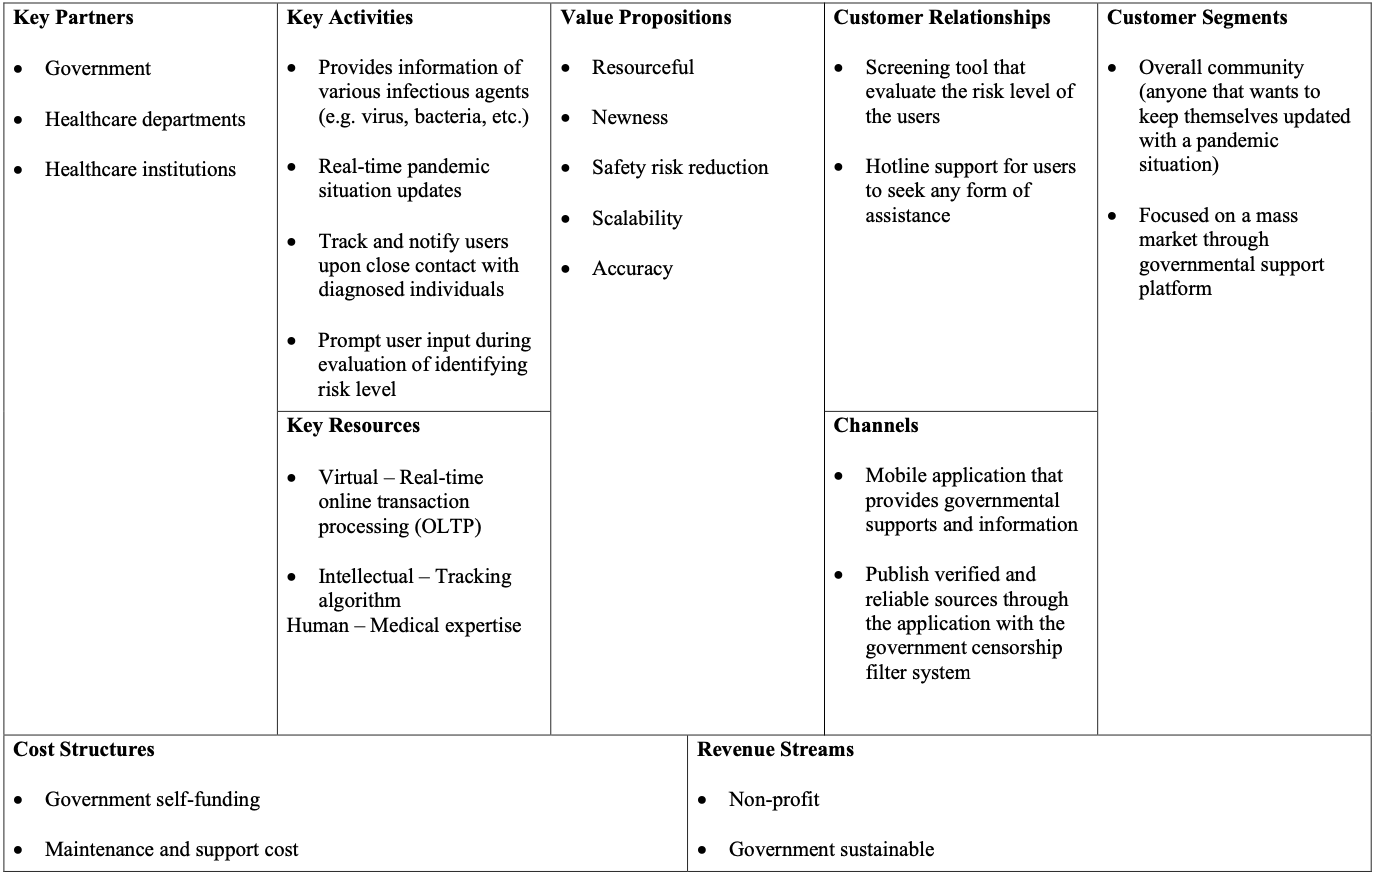
\includegraphics[width=\linewidth]{img/bmc.png}
        \caption{Business Model Canvas}
        \label{fig:bmc}
      \end{figure}
    
    \subsubsection{Paper prototyping}
      \par This approach is a method to quickly visualize the conceptual designs that could be a wireframe for
      the digital interfaces. A total of 9 simple interfaces of low-fidelity wireframes were created to
      showcase the general functionalities through the proposed solution interfaces.
      \begin{figure}[H]
        \centering
        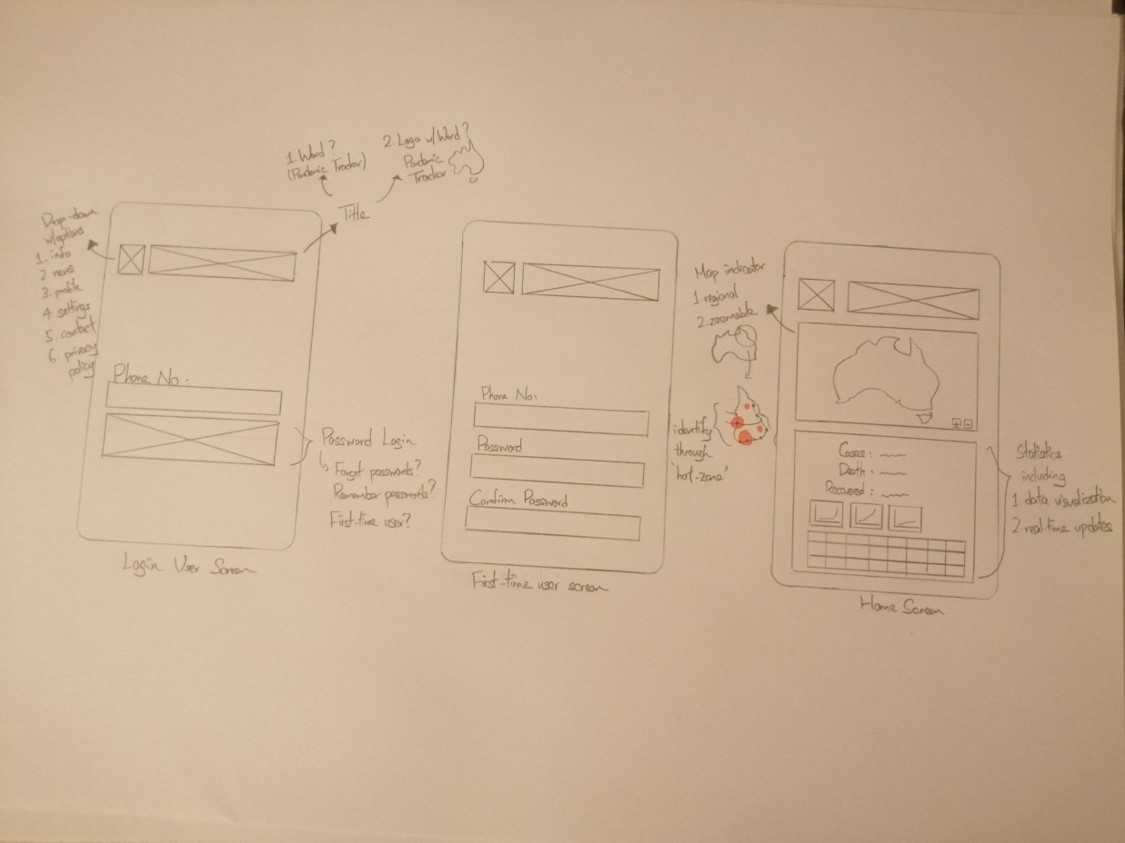
\includegraphics[width=\linewidth]{img/low-fidelity-prototype/sketch-1.png}
        \caption{Login, Register and Home Screen}
        \label{fig:prototype-01}
      \end{figure}
      
      \par Based on Figure \ref{fig:prototype-01}, the wireframe consists of the login, register, and home screen interfaces, A valid phone number, and a password are required for login. For first-time users, the login screen will have a link directing the user to the register screen to fill in the phone number and password to register as a member. Account recovery methods such as password reset will be included if the users forget their password. The home screen would include a heatmap indicator with statistical data of regional information including zone safety level, statistics, distribution of cases (orange dots in color).
      
      \begin{figure}[H]
        \centering
        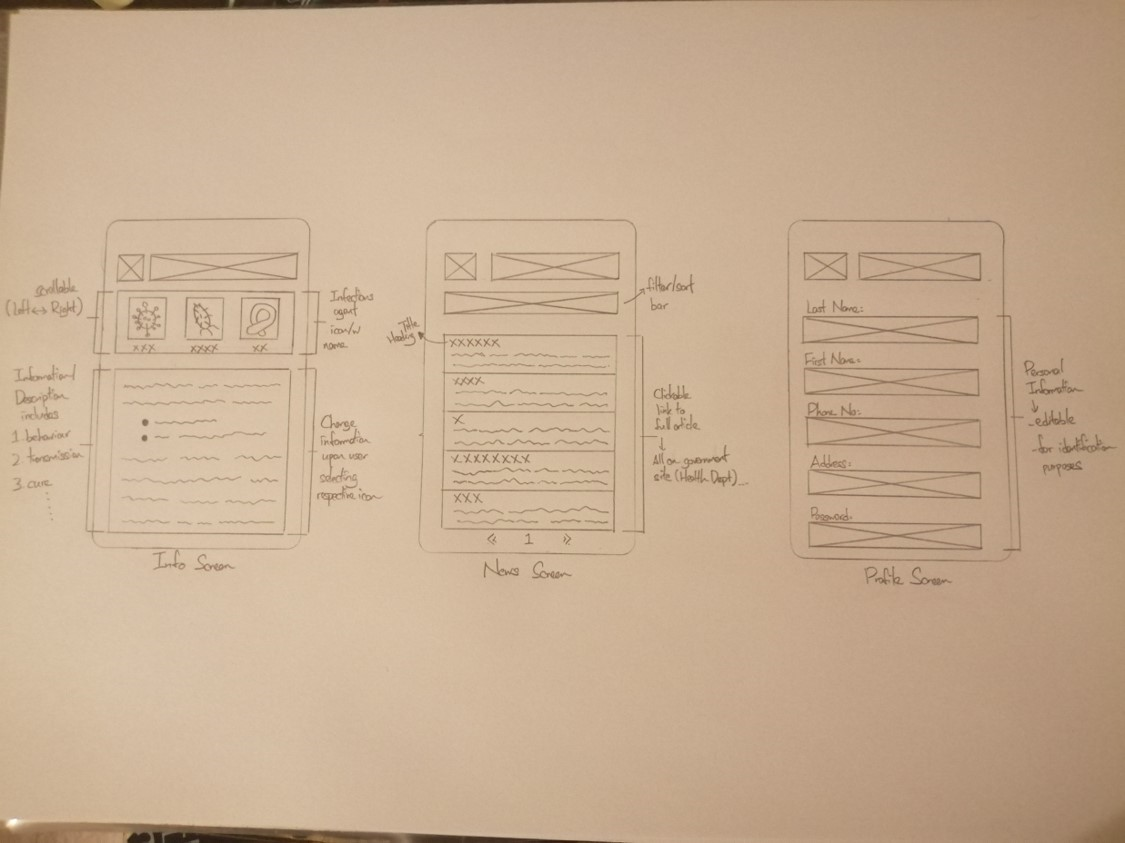
\includegraphics[width=\linewidth]{img/low-fidelity-prototype/sketch-2.png}
        \caption{Info, News and Profile Screen}
        \label{fig:prototype-02}
      \end{figure}

      \par Figure \ref{fig:prototype-02} shows the information, news, and profile screen. Basic information of the infectious agents will be explained in layman terms which includes behavior, characteristics, transmission, and more. The following news screen is updated with the latest articles from verified publishers for any international and domestic news. The profile screen will display basic information consists of the authentic name of the user, phone no, and home address, which is crucial when immediate quarantine or government support is needed.

      \begin{figure}[H]
        \centering
        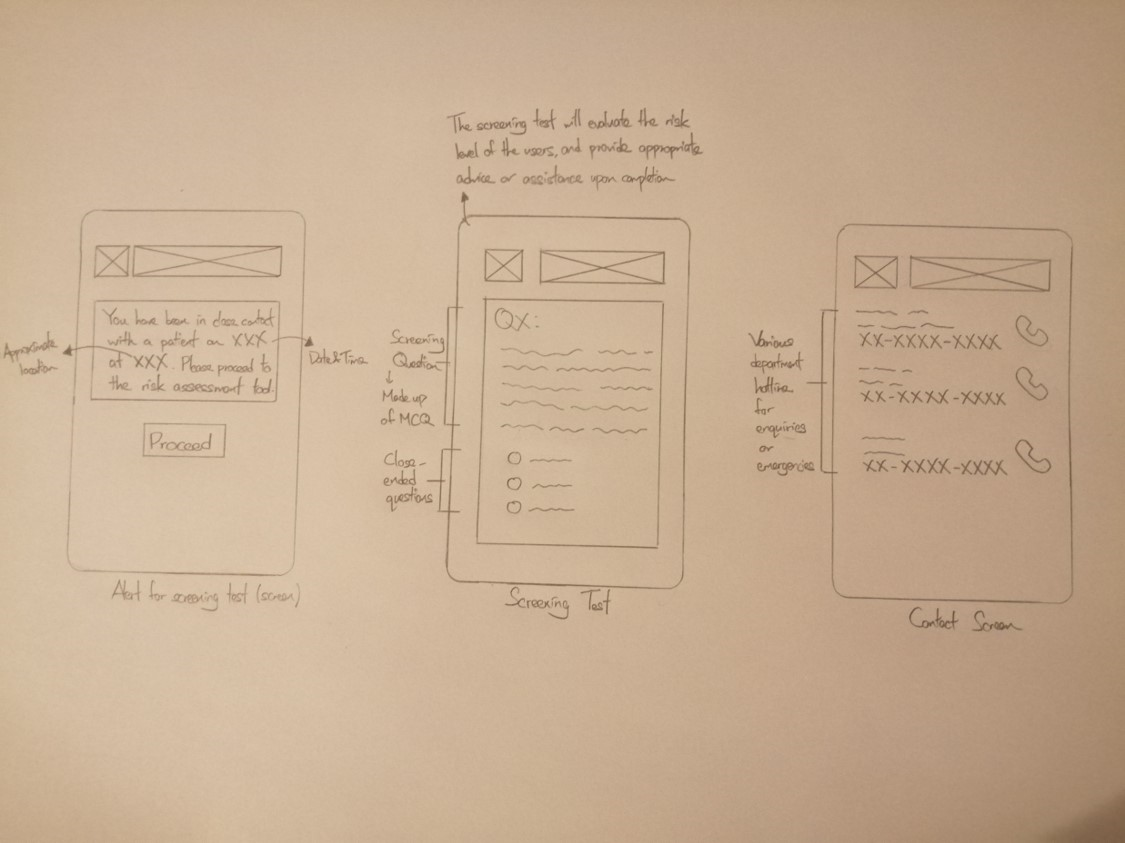
\includegraphics[width=\linewidth]{img/low-fidelity-prototype/sketch-3.png}
        \caption{Notification, Q\&A and Contact Screen}
        \label{fig:prototype-03}
      \end{figure}
      
      \par An alert notification, screening test, and contact screen is shown in Figure \ref{fig:prototype-03}. The alert notification would pop up when the user has been verified having close contact with a diagnosed individual. The user will then be prompted to proceed to the Q\&A panel for a short evaluation. The result will display the user's personal risk level, which may or may not necessarily to request medical support. Apart from this, the contact screen is listed with relevant government hotlines that could be helpful for inquiries or emergencies directly.

    \subsubsection{Digital Prototyping}
      \par This approach is to create a high-fidelity sketch for multiple user interfaces. A wireframe is built upon
      a mixture of simulations contents with including basic design components. The current digital
      prototypes do not focus on the main functionalities of how a pandemic tracking application should
      operates. However, it focused on finding elements and concepts that could be included by studying
      user behavior through usability testing to increase the adoption and retention rate of the application.

      \begin{enumerate}[a)]
        \item \textbf{Iteration 2}
        \begin{enumerate}[label=(\roman*)]
          \item \textbf{Map Simulation}
            \begin{figure}[H]
              \centering
              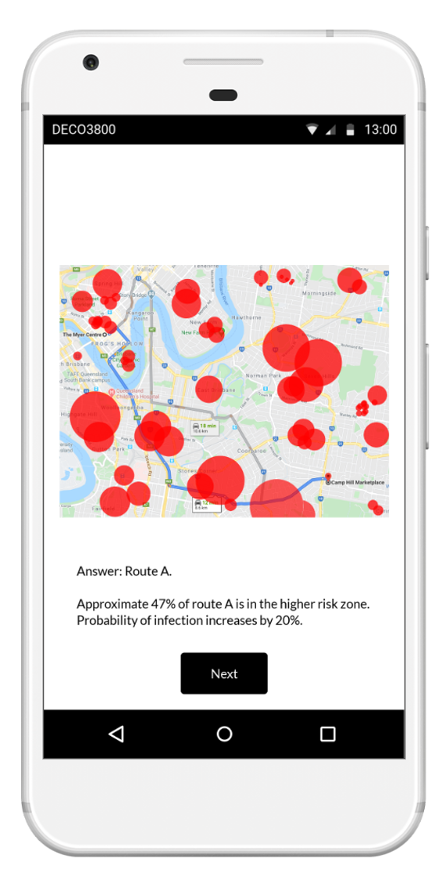
\includegraphics[scale=1]{img/digital-prototype/map-simulation.png}
              \caption{Map Simulation}
              \label{fig:digi-proto-01}
            \end{figure}
            \par The above Figure \ref{fig:digi-proto-01} simulation was proposed as a part of the product goals to improve decision making in risk assessment during traveling. Moreover, this simulation is integrated with the real-time heat map generated from the COVID-19 statistics. This algorithm will be included to calculate the user infection rate throughout the planned journey which happens to be in the hot zone when traveling.
            \par This simulation could act as a supplementary tool for helping users to make sound judgment to consider their surrounding loved ones as well. This could also invoke empathy among the users and therefore encourages it for journey planning, thus, help users to build a stronger relationship with their loved ones during this pandemic period.
          \item \textbf{Quarantine Life Simulation}
            \begin{figure}[H]
              \centering
              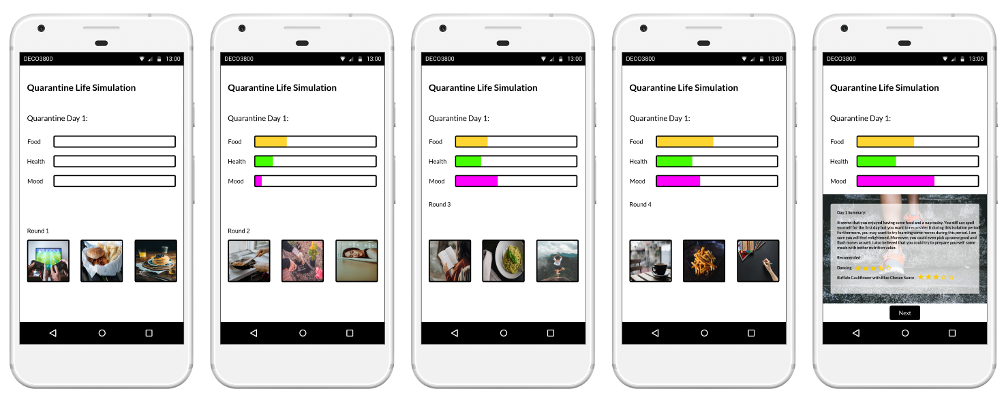
\includegraphics[scale=1]{img/digital-prototype/quarantine-life.png}
              \caption{Quarantine Life Simulation}
              \label{fig:digi-proto-02}
            \end{figure}
            \par The above Figure \ref{fig:digi-proto-02} simulation through cognitive learning was proposed as a part of the product goals to promote a healthier lifestyle during this pandemic period. Moreover, this simulation implemented via gamification by selecting a desired picture through each round daily. The food, health, and mood barometers are each an attribute representation of eating habits, vitality, and mental state. The system will then analyze the user behavior and provide a summary according to the user selection including the total percentages in the barometers. The summary will include the users' behavioral patterns and provide recommendations to improve certain attributes. Hence, this simulation could help encourages habits and behaviors change during this pandemic period for users to adopt a healthier lifestyle for low-stress living.
          \item \textbf{Simulations Removal}
            \par In the final presentation for Iteration 2, our team receive critiques from the mentors and peers regarding the obscurity of our product positioning as a pandemic tracking application. As our goals set were trying to include more features in other aspects such as learning with how the typical pandemic tracking applications (e.g. Australia COVIDSafe, Singapore TraceTogether) did not provide, it was more of a benefit-focused positioning for the product. However, after we realize how both COVIDSafe and TraceTogether has not been very successful through in-depth research, we found out there is a barrier for users to ``trust" their data and privacy with us. Hence, we changed our product goals approach which is a behavior-based positioning. With this approach, we focused on building trust with users that the application may evoke such a feat to increase users' participation and engagement with the application. In other words, we do not further include educational simulations that are not aligned with our product goals that deliver the core value of building ``trust" with the user.
        \end{enumerate}
        \item \textbf{Iteration 3}
          \par The below figures will display the functionalities of our final proposed solution to deliver the core
          values as a pandemic tracking application.
          \begin{figure}[H]
            \centering
            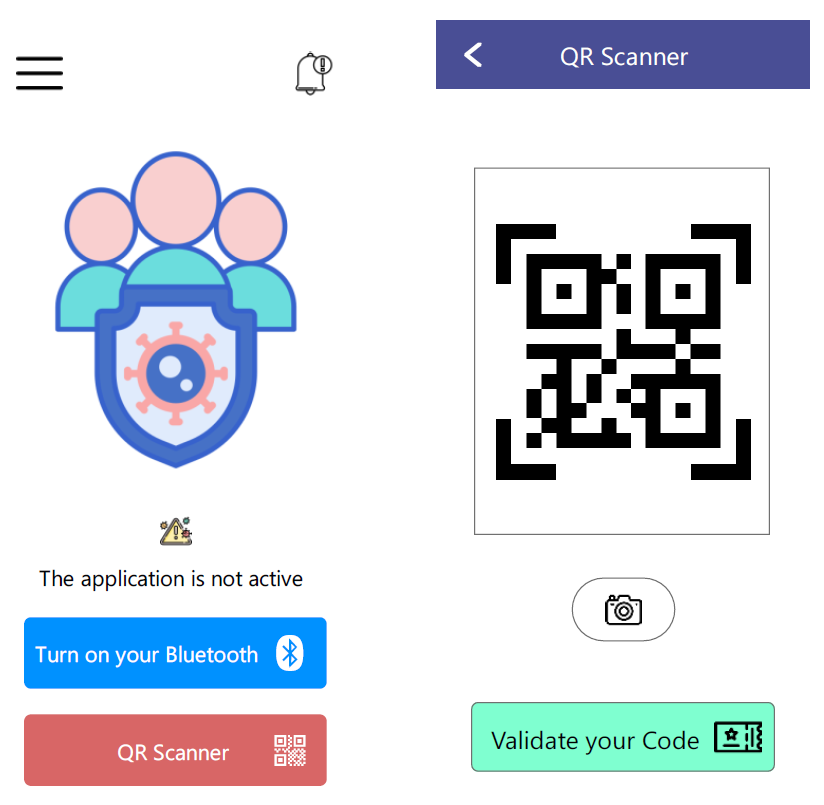
\includegraphics[scale=1]{img/prototype/iter3-proto-1.png}
            \caption{Main Screen and QR Code Scanner Screen}
            \label{fig:iter3-proto-1}
          \end{figure}
          \par According to figure \ref{fig:iter3-proto-1}, the left screen displayed the two main functionalities of the application, which
          are the Bluetooth status and the QR Scanner. If the Bluetooth is deactivated, a button with be
          prompted with a message ``Turn on your Bluetooth" that will direct the users to the Settings screen to
          activate it once pressed. Besides that, while being at outdoors, the users would need to scan the QR
          Code to access certain areas or zones through tapping on the ``QR Scanner" button. After that, a screen
          shown as the right of figure \ref{fig:iter3-proto-1} will provide the users with two options, either by scanning the code via
          camera or authenticating the scanned code validity via the ``Validate your Code" button.
          \begin{figure}[H]
            \centering
            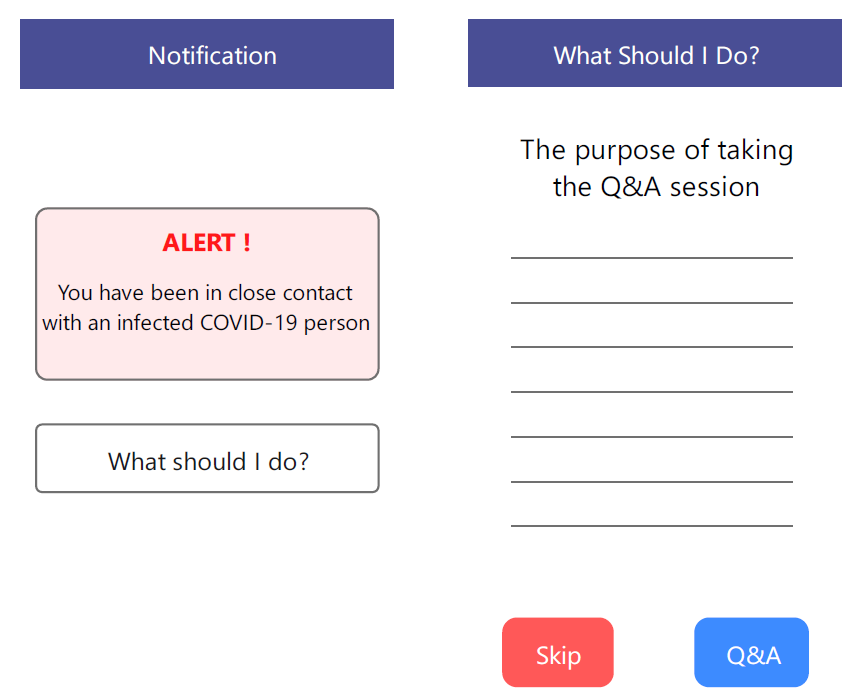
\includegraphics[scale=1]{img/prototype/iter3-proto-2.png}
            \caption{Notification and Screening Test Guideline Screen}
            \label{fig:iter3-proto-2}
          \end{figure}
          \par Based on figure \ref{fig:iter3-proto-2}, the left screen displayed a message notifying the user when had been close contact
          with a positively tested individual. The notification system is one of the core features that the
          application delivers its core values to the user. The user could only navigate to the right screen shown
          in figure \ref{fig:iter3-proto-2} through tapping on ``What should I do?" button. It will then allow the user to know more
          about the purpose of proceeding with the Q\&A session to receive advice from the health authorities.
          However, the user has the options whether to proceed or not either ignoring it by tapping the skip
          button or proceeding the session by the Q\&A button. The user can still access the right screen of
          figure \ref{fig:iter3-proto-2} via the notification icon on the top left corner of figure \ref{fig:iter3-proto-1} left screen.
          \begin{figure}[H]
            \centering
            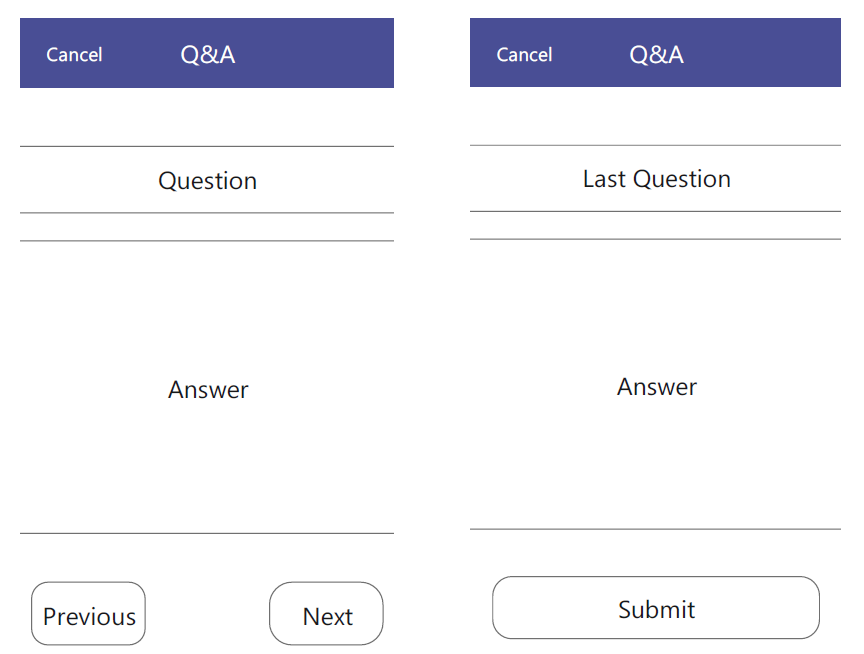
\includegraphics[scale=1]{img/prototype/iter3-proto-3.png}
            \caption{Notification and Screening Test Guideline Screen}
            \label{fig:iter3-proto-3}
          \end{figure}
          According to figure \ref{fig:iter3-proto-3}, the left screen is the screening test screen after the user agreed to participate in it by tapping the Q\&A button to the right of the figure \ref{fig:iter3-proto-2}. The screening test consists of several questions without any questions that need any demographic and geographic information input by the user. A user can decide to opt-out the test anytime via the ``Cancel" button on the top-left corner of figure \ref{fig:iter3-proto-3} left screen. Moreover, the user could skip any questions through the ``Next" button and navigate to the previous question through the ``Previous" button. The right screen of figure \ref{fig:iter3-proto-3} is the submit screen for the screening test. The user could complete the test by tapping on the ``Submit" button. All the data is then recorded and redirects back to the main screen.
          \begin{figure}[H]
            \centering
            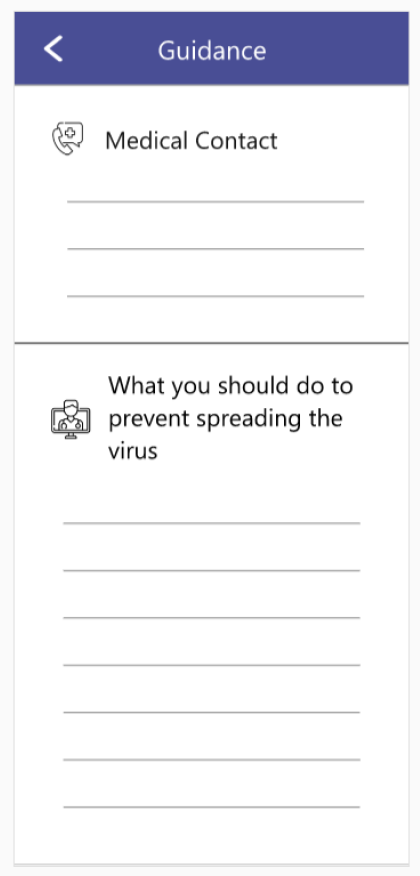
\includegraphics[scale=1]{img/prototype/iter3-proto-4.png}
            \caption{Support Screen}
            \label{fig:iter3-proto-4}
          \end{figure}
          Based on figure \ref{fig:iter3-proto-4}, it is a support screen that provides numerous support channels to guide and help any users in need. The User Guidance screen would include essential categories such as medical contacts and prevention measures. If a user needs a list of emergency and health support hotlines, they could tap on the Medical Contact section. The purpose of this implementation is to provide users a readily accessible way to receive the support they need. Moreover, if the users are unsure how to keep themselves protected and prevent further transmission of the virus, they could explore the suggestions section that provides detailed instructions for the prevention measures.
          \begin{figure}[H]
            \centering
            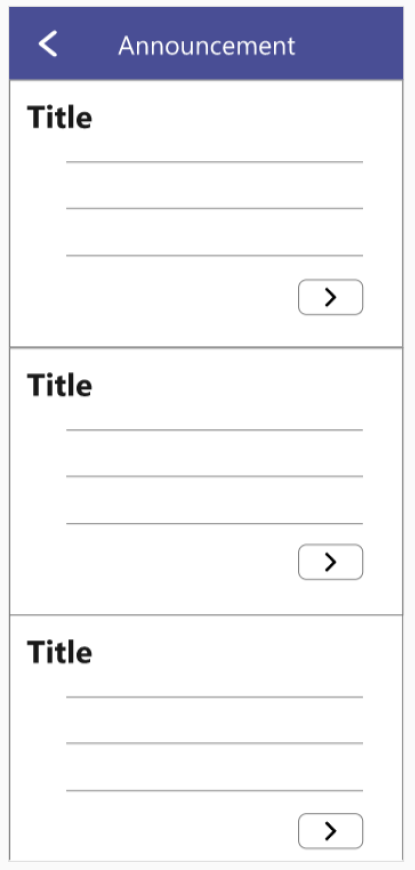
\includegraphics[scale=1]{img/prototype/iter3-proto-5.png}
            \caption{Announcement Screen}
            \label{fig:iter3-proto-5}
          \end{figure}
          \par According to figure \ref{fig:iter3-proto-5}, the application will provide official announcements from the government and
          authorized organizations to the users as a part of user support. This page is expected to be informative,
          genuine, and in real-time so that the users could frequently keep track of the latest pandemic updates.
          This implementation is included in the User Support section.
          \begin{figure}[H]
            \centering
            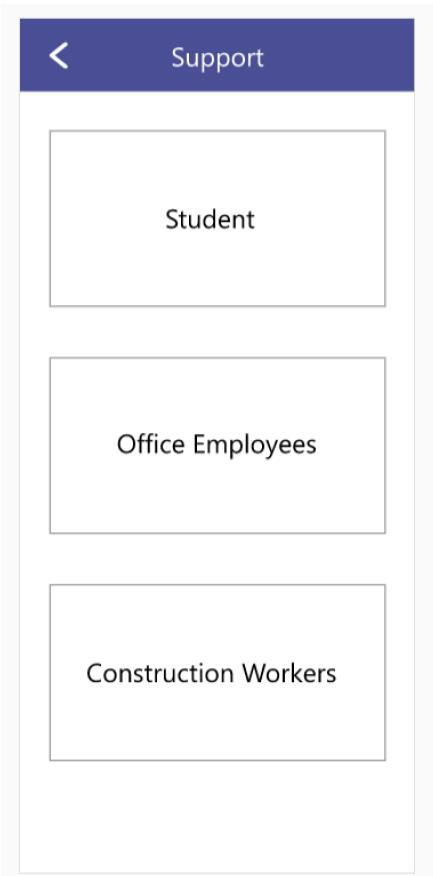
\includegraphics[scale=1]{img/prototype/iter3-proto-6.png}
            \caption{User Support Package Screen}
            \label{fig:iter3-proto-6}
          \end{figure} 
          \par Based on figure \ref{fig:iter3-proto-6}, each respective target audience would receive different support packages from the
          application. In specific, the User Support section would display a wide range of categories
          corresponding to groups of users affected by the pandemic such as students, office employees and
          construction workers. Any other target stakeholders could be included in any further research by
          another team but not in the last milestone. By tapping on a tab corresponding to the appropriate
          user category, the users could explore valuable assistance packages recommended by the application.
          \begin{figure}[H]
            \centering
            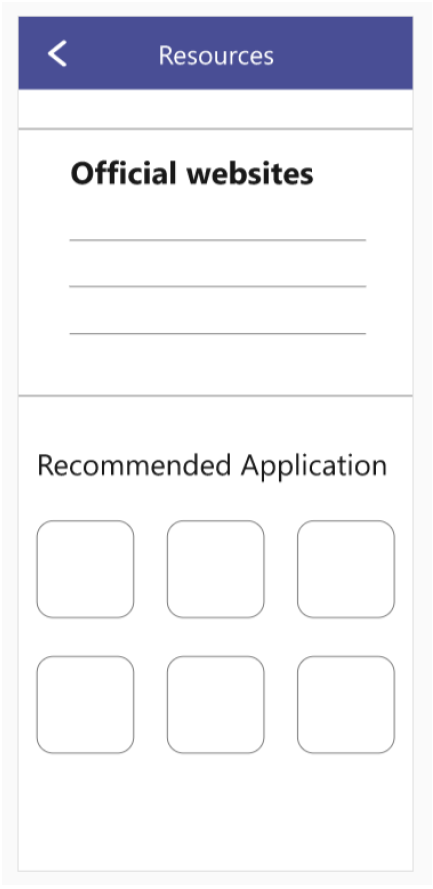
\includegraphics[scale=1]{img/prototype/iter3-proto-7.png}
            \caption{Resource Screen}
            \label{fig:iter3-proto-7}
          \end{figure}
          \par According to figure \ref{fig:iter3-proto-7}, the final step will proceed with the application suggesting useful resources to help users stay healthy physically and mentally. On the Resources page, the users could find essential information about the pandemic such as virus spreading prevention techniques through official websites of government agencies and departments. This section also recommends associated applications that help users to cope with multiple issues during the quarantine.
      \end{enumerate}

  \subsection{Behavioral Design}
    \par Behavioural design is used as a reference and guideline to identify the user behavioral pattern of a
    common majority community towards digital data sharing. This is to study how a user's decision may
    be influenced by the common majority community of other people. The study helps us to understand
    how certain design components could be included and designed to increase user participation and
    engagement rate for the application to achieve our product goals. Hence, we integrate the behavioural
    design principles into our proposed solution.

    \subsubsection{Behavioral Modelling}
      \begin{figure}[H]
        \centering
        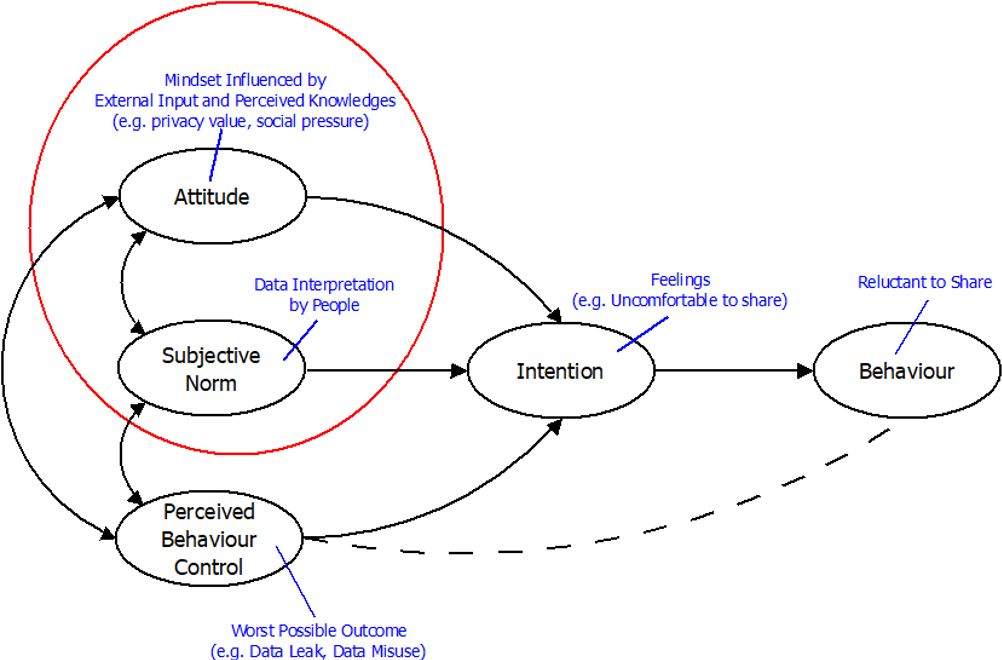
\includegraphics[scale=1]{img/digital-prototype/behavior-model.png}
        \caption{Data Sharing Behavior Model}
        \label{fig:behavior-model}
      \end{figure}
      \par This modeling concept template is borrowed and remodeled from \parencite{Ian8}. The above figure \ref{fig:behavior-model} hows the
      modelling with my notation on how data privacy has been perceived by the general public in current
      times. From the current public behavior towards a deployed pandemic tracking mobile application,
      most of them are reluctant to share their data and do not find it helpful. This is mostly affected by
      how they perceived the worst possible outcome interpreted by the public eye or based on their own
      knowledge. Hence, it may further influence other peoples' perspectives collectively known as
      collective consciousness. This may create norms that are misleading for other people through social
      pressure as well. In other words, we would like to implement some behavior design principles for
      our application to change the people's attitude that would not be influenced by the current subjective
      norms created for digital data sharing (red circle shown above).
    
    \subsubsection{Behaviour Design Example}
      \begin{enumerate}[a)]
        \item \textbf{Iteration 2}
          \begin{figure}[H]
            \centering
            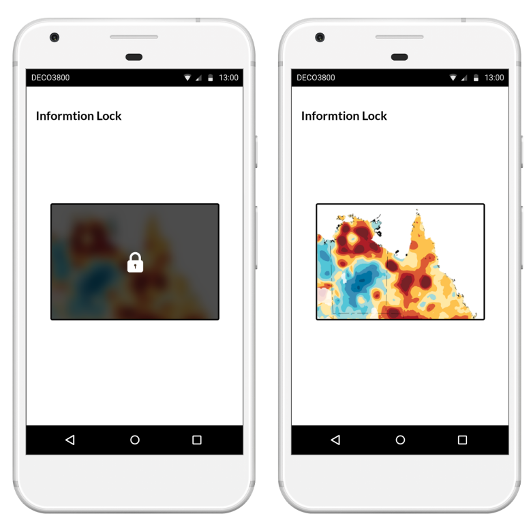
\includegraphics[scale=1]{img/digital-prototype/info-lock-screen.png}
            \caption{Sequential Information Release Example}
            \label{fig:digi-proto-03}
          \end{figure}
      \end{enumerate}

      \par From the above Figure \ref{fig:digi-proto-03}, it displayed an example for the Queensland regional COVID-19 hot zones through a heatmap illustration. The information on the left is locked while unlocked on the right. This design had applied a concept called sequential information release. This approach is to limit the disclosure of sensitive data and information to the application users. Moreover, it is equally important and fair to all users when certain users are providing necessary information while others are taking for granted. In such cases, we do not imply consent to any users who are not sharing their information while protecting the privacy of other users who shared their information. Thus, it promotes a scenario of user inducing altruistic behavior known as reciprocal altruism. In other words, we study the user psychology to create guidelines and implement behavior design principles into our application which could elevate user experience that could positively impact their mindset of how our application perceive user’s privacy and promote the element of trust to the users.
      \par \textbf{Final Decision}: The team decided to remove the above-mentioned design principle during the end of Iteration 2.
      When aligning our product goals set for Iteration 3, we decided to promote trust using a very different
      approach for the data algorithm (e.g. black box) to store user data, which involves cryptography that
      is not disclosing information without user consent. Hence, the mentioned behavioral design is not
      applicable as there is not information display unless invoked by a scenario (explained in Digital
      Prototyping at Iteration 3). Moreover, the sequential release would not be relevant for Iteration 3 as the
      information will need to display as a whole without leaving out any segmented or fragmented
      information. So, it is not possible to use such a method to provide data protection for our application.

  \subsection{Usability Testing}
    \par The purpose of usability testing is to evaluate a product through a developed prototype based on the feedbacks collected from the users. It helps to refine user requirements and visual designs of the product throughout the development cycle. Moreover, it focused on how the users interact with the prototype, completes the given tasks, and observe the users during testing. It could collect valuable insights through learning the user’s behavior and preference from the user testing. Thus, the insights could further improve the prototype for iterative testing sessions.
    \par The prototypes used for the testing sessions are the map simulator and quarantine life simulator. All the participants joined have given their consent for the testing session. The testing is conducted through a link to the prototype through real-time communication via video or phone calls with the participants.
    
    \subsubsection{Retrospective Think Aloud (RTA)}
      \par This technique requires participants to retrace their steps when the session is complete. This technique
      is particularly useful to verbalize the participant's thoughts and embed the process into their memory.
      Hence, it could check whether the participants could visualize the contents during memory tracing,
      which indicates how the visual content impression is delivered to them during the session. In other
      words, the user preferences and behaviors would influence how they perceived the simulation
      prototype values and core processes delivered to them.
      \par \textbf{Findings}:
      \begin{itemize}
        \item Map Simulator:
          \begin{itemize}
            \item 4 of 5 participants think that the information is insufficient for convincing them from leaving the house.
            \item All participants do not remember the major hot zones after answering it.
          \end{itemize}
        \item Quarantine Life Simulation:
          \begin{itemize}
            \item 3 of 5 participants spent a longer average time testing the quarantine life simulator.
            \item 3 of 5 participants think that the quarantine life simulator is a fun-to-play game only.
          \end{itemize}
      \end{itemize}
    
    \subsubsection{Concurrent Probing (CP)}
      \par This testing technique requires participants to work on the tasks given and asking follow-up questions
      when the participants engaged in the session. This technique is suitable to prompt real-time feedback
      on each task executed, which could directly project their current feelings towards the prototypes.
      In other words, we could understand the user psychology path when carrying out tasks through how
      the application may evoke different feelings towards the user or through the user behavior in
      performing tasks on the application. Hence, it creates a minimum threshold on how these
      functionalities could provide its usefulness to increase user retention rates through the testing session.
      \par \textbf{Findings}:
        \begin{itemize}
          \item Map Simulator:
            \begin{itemize}
              \item All members suggested for more travel options. 
              \item 3 of 5 participants suggested to include information as hints when they think it is good and easy to reference for authentication.
            \end{itemize}
          \item Quarantine Life Simulation:
            \begin{itemize}
              \item 2 of 5 participants think that the selection rounds could be increased for a more thorough representation of their daily lifestyle.
              \item 4 of 5 participants think that the selected categories for each round in the quarantine life simulator are inconsistent. 
            \end{itemize}
        \end{itemize}

    \subsubsection{Insight Summary}
      \begin{enumerate}[a)]
        \item \textbf{Iteration 2}
        \begin{itemize}
          \item Map Simulator:
            \begin{itemize}
              \item More statistical inputs are required to increase user interest and authenticity from verified sources. 
              \item Participants are likely wanting to travel in their own preferred transport only, which the current simulator only displays one option traveling by car only. In other words, this may happen due to habit issues or lack of confidence traveling with a non-preferred vehicle during this period.
              \item Create important visual components to be more appealing and attractive for developing as a semantic memory during memory encoding (Behavioural design principles).
              \item Providing minor support as guidelines such as nudge could its memory point for user impression.
            \end{itemize}
          \item Quarantine Life Simulation:
            \begin{itemize}
              \item Create selection within the category in each round for better memory tracing.
              \item Providing selection pictures that are more approximate to local culture and habits accordingly.
              \item More in-depth analysis of the daily summary should be carried out with the prompted input.
              \item Participants tend to spend more time for recalling and retracing memory with the selection pictures each round, indicating the significant values as an additional component to increase retention rate.
            \end{itemize}
        \end{itemize}
      \end{enumerate}
\section{Plan}
  \subsection{Possible Privacy-Preserving Laws/Technologies}
    \par User privacy is a fundamental human right. Coercing people into turning the GPS on and granting their Location access to the third-party application all the time is not the right thing to do. One of the proposed solutions is convincing users that all collected data will be encrypted and send to the Government only, anyone else, even though developers cannot know exactly where they are and where they were.
  \subsection{Accuracy of Technologies}
    \par Since the behavior of the virus varies depending on different conditions (e.g. type of surface, temperature or humidity of the environment) \parencite{Plan3}, it is an arduous task to know exactly how long the virus lasts outside the host. A solution for this is when knowing that an infected person went to a specific place in the past, the mobile application would push notification to all the people within 5 kilometers radius with real-time tracking since the day that infected person came to until 72 hours later \parencite{Plan4}. Hence, all notified people would raise the awareness of limiting on surface touching and regularly washing their hands with an alcohol-based hand rub or wash them with soap and water.
    \par According to a study published last year \parencite{Plan1}, a phone is typically able to determine its position with an accuracy between 7 and 13 meters in urban areas. However, it is recommended that people should keep 1.5 meters away from others as much as possible is one of the ways proposed by Social distancing (also called physical distancing) to help slow the spread of viruses \parencite{Plan2}. Therefore, the accuracy of the GPS of a mobile phone radically affects the results of distancing among people even though they are not in that close contact with each other (within 1.5 meters). In order to tackle this problem, what our application could do is sending the data to the Government only then they would decide how these data might be handled: Maybe they would do nothing, or give warning to the people who were in close contact with the infected person about quarantining at home in 14 days. Furthermore, cooperating with third-party services such as Translink would make a great contribution to the tracking system of our project. For instance, if there was a person who was infected with COVID-19 came to a bus, Translink could get access to his/her Go card in order to track which bus they took in recent days then the company would sterilize that specific bus and send back information to us to notify all associated people who took the same bus with the COVID-19 patient. Another feasible solution to tackle the problem of accuracy is by using short-range Bluetooth signals from other’s smartphones. The biggest advantage of this application compared to other existing ones is the combination of location services and Bluetooth signals. With GPS, the system can track the areas where the person who tested positive for the virus came with the purpose of minimizing the spread of the virus outside the host. Moreover, thanks to Bluetooth, the system could identify people who were in close contact with that patient and then push a notification to them about what to do next. Supposing when a person is required to self-quarantine at home, the application would frequently interact with that person via Q\&A sections and provide emergency contact to medical services in case of unwell health conditions. In addition, the GPS, as well as Bluetooth signal, are needed to be accessed all the time, included in and after lockdown to reduce the pandemic outbreak.
  \subsection{Conclusion}
    \par The purpose of this application is health communication. However, location accessibility is the key to the success of this application. Our application could be gotten the most to prevent the pandemic if there were cooperation among inhabitants to get access to their location for real-time tracking. The situation was put on high alert if there was a person who infected with COVID-19 did not turn GPS and Location Services on their mobile phone and then entered public places (e.g. Supermarket, City center). In consequence, whoever entered those places within 3 days might acquire the virus after touching contaminated objects or surfaces.


\section{Team Reflection}
  \par There is no doubt that COVID-19 has made a lot of impact on our team's efficiency. It can be said that in order for a team to perform at its best, there is a need for direct interaction between team members. Fortunately, five out of six members in our team live in the same student accommodation which is our advantage over other teams. We could easily meet each other and discuss when there was a need to revise the project. But it was not for that reason that we did not have online meetings every week to update the status of the assignment. We had a weekly meeting on Zoom after every studio class to further discuss our ideas. Even in weeks without studio classes, we still tried to hold a meeting by ourselves so that we could accelerate the progress of our project. Our team also created a shared folder on Google Drive and a private channel on Slack. The folder was where we uploaded all the important files namely reports, clips of the presentation, and notes. The Slack channel was our main means of communication. All the crucial announcements would be posted on this channel so that the team members could keep up with the flow of the project. Besides, we used the channel to share recent articles, reports or any literature that was relevant to our problem space and solution. 
  \par At the beginning of each meeting, we would make time for each person to present shortly what they had researched in that week. We utilized the whiteboard and screen sharing on Zoom to take notes during the meetings. Once everyone in the team was done presenting, we moved on to solving problems still present in our model. At the same time, we also revised the comments from our tutors and classmates on the project. These comments were very valuable as they provided us with a more objective perspective on the issues. Moreover, they helped us better understand the users’ needs and expectations. Before any meeting ending, we divided the work based on the requirements of the next assessment item. A team-only deadline was always set to guarantee that our work would not be delayed. In the end, all the notes that had been taken during the meetings were posted to our Slack channel for later reviewing. Although our project is far from being perfect and there are still many issues that we have to tackle, everyone in the team has put in their best effort to develop the project up to the point where it is right now. Healthcare, which is the primary topic that our application concerns, is not our major yet we still did try to gain as much knowledge as possible in this field and of course in the software technical field as well. The evidence is that each member was fully responsible for the part they were assigned. We also adhered to the rules set out to make sure the group works the most effectively.
  \par Nevertheless, in spite of our appropriate and logical teamwork etiquette as well as everyone's devotion to the success of the project, there were still a few difficulties that went against our will:
    \begin{itemize}
      \item The fact that English is everyone's second language occasionally made it fairly difficult to express and understand each other's ideas due to the difference in our speaking accents and ways of phrasing. To overcome this problem, all of us had to pay close attention and be patient whenever a member was speaking up his ideas or opinions. 
      \item As the semester had moved fully online, networking issues were undoubtedly another difficulty we had to face. Sometimes someone in the team could not catch up with the online meeting discussion because of weak Internet stability. To solve this, we either needed to repeat things multiple times or recorded the entire meeting for later review. In the worst case which is not having an Internet connection (which happened to the five of us who live in the same student accommodation as the Internet provider was going through some maintenance at the time of studio meeting), we had to use our 4G mobile data as an alternative.
      \item Although having five out of six members living under the same accommodation has already been a great advantage for our team, communications via online media with the one other member were sometimes challenging as online messages obviously do not get acknowledged immediately similar to the way that face-to-face conversations do. Therefore, we had to exchange mobile phone numbers in case the other member needed to be notified of any urgent information.
    \end{itemize}
  \par All in all, despite all of the difficulties and challenges our team had to face and find a way to overcome throughout the development of the project, we all feel satisfied with how we have functioned as a team as well as the final solution that we have managed to deliver. We are all confident to admit that our operation was acceptably seamless, which lives up to the name of our team - United.   
\newpage

\begin{appendices}
  \section{Quantitative Research – Survey} \label{appendix:quantitative}
  
    \begin{figure}[H]
      \centering
      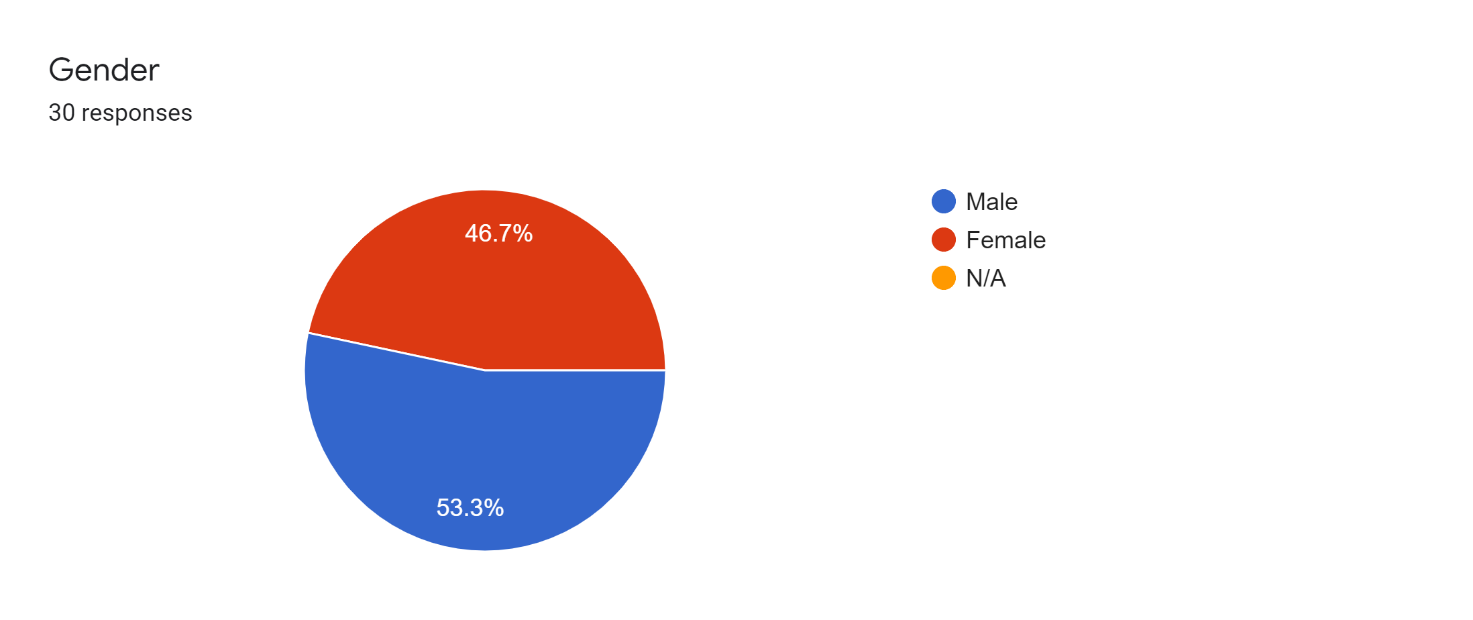
\includegraphics[width=18cm]{img/Survey/Q1.png}
      % \caption*{#3}
    \end{figure}
    \begin{figure}[H]
      \centering
      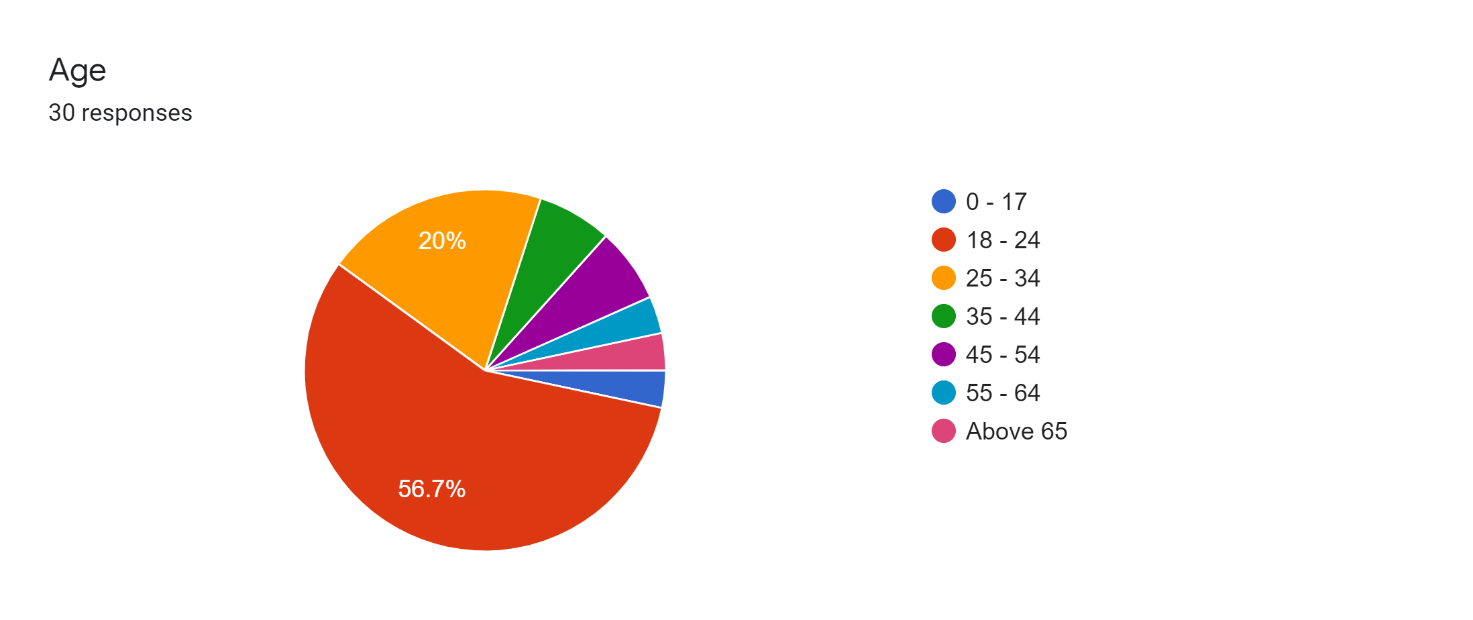
\includegraphics[width=18cm]{img/Survey/Q2.png}
      % \caption*{#3}
    \end{figure}
    \begin{figure}[H]
      \centering
      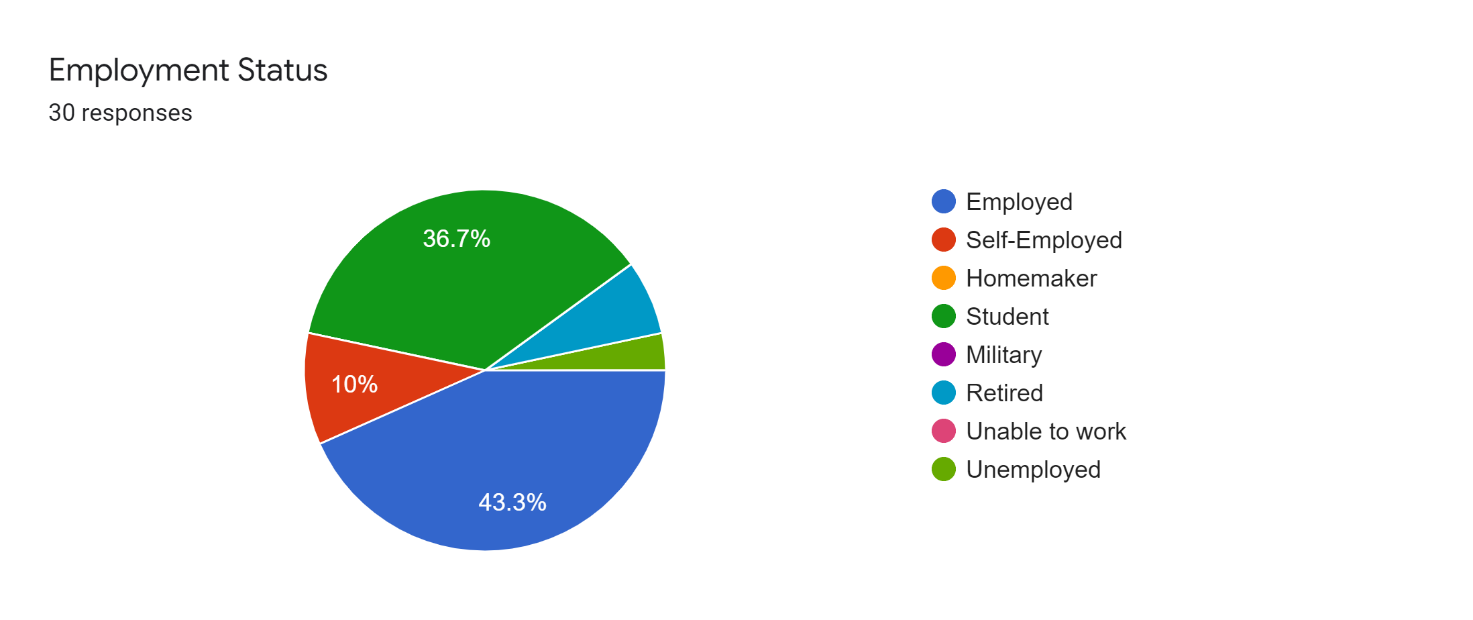
\includegraphics[width=18cm]{img/Survey/Q3.png}
      % \caption*{#3}
    \end{figure}
    \begin{figure}[H]
      \centering
      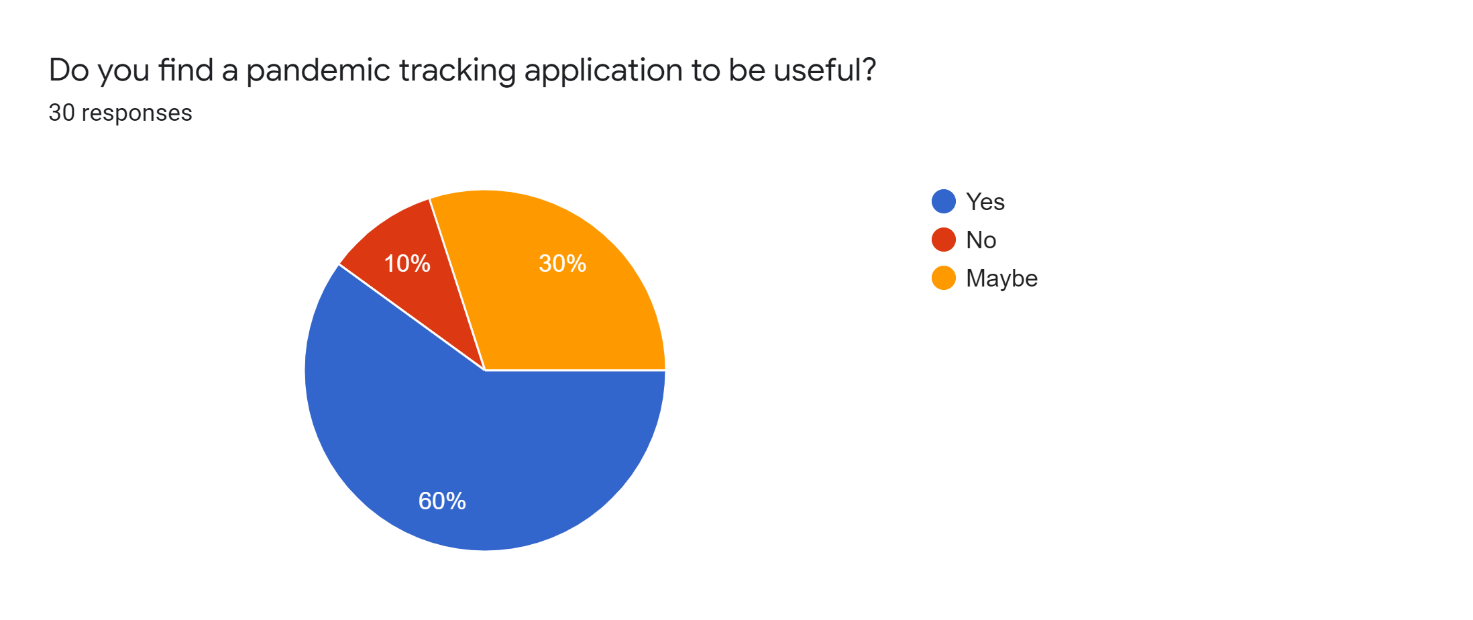
\includegraphics[width=18cm]{img/Survey/Q4.png}
      % \caption*{#3}
    \end{figure}
    \begin{figure}[H]
      \centering
      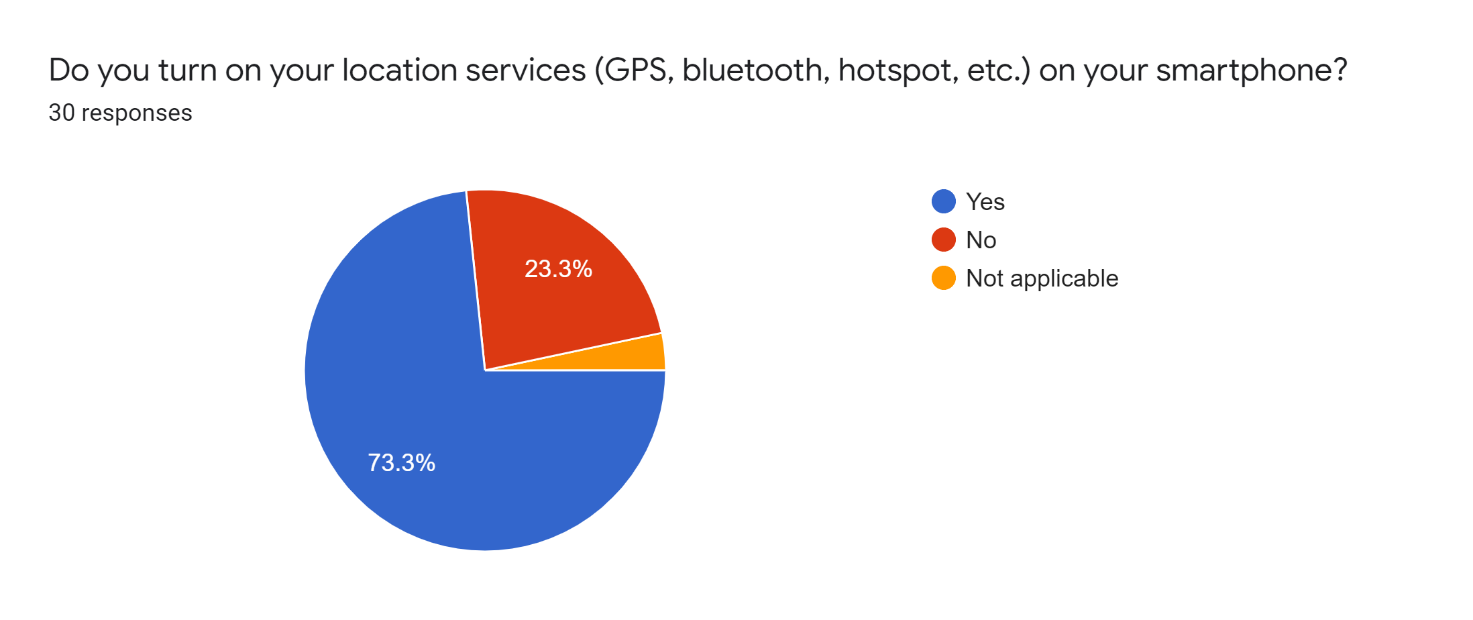
\includegraphics[width=18cm]{img/Survey/Q5.png}
      % \caption*{#3}
    \end{figure}
    \begin{figure}[H]
      \centering
      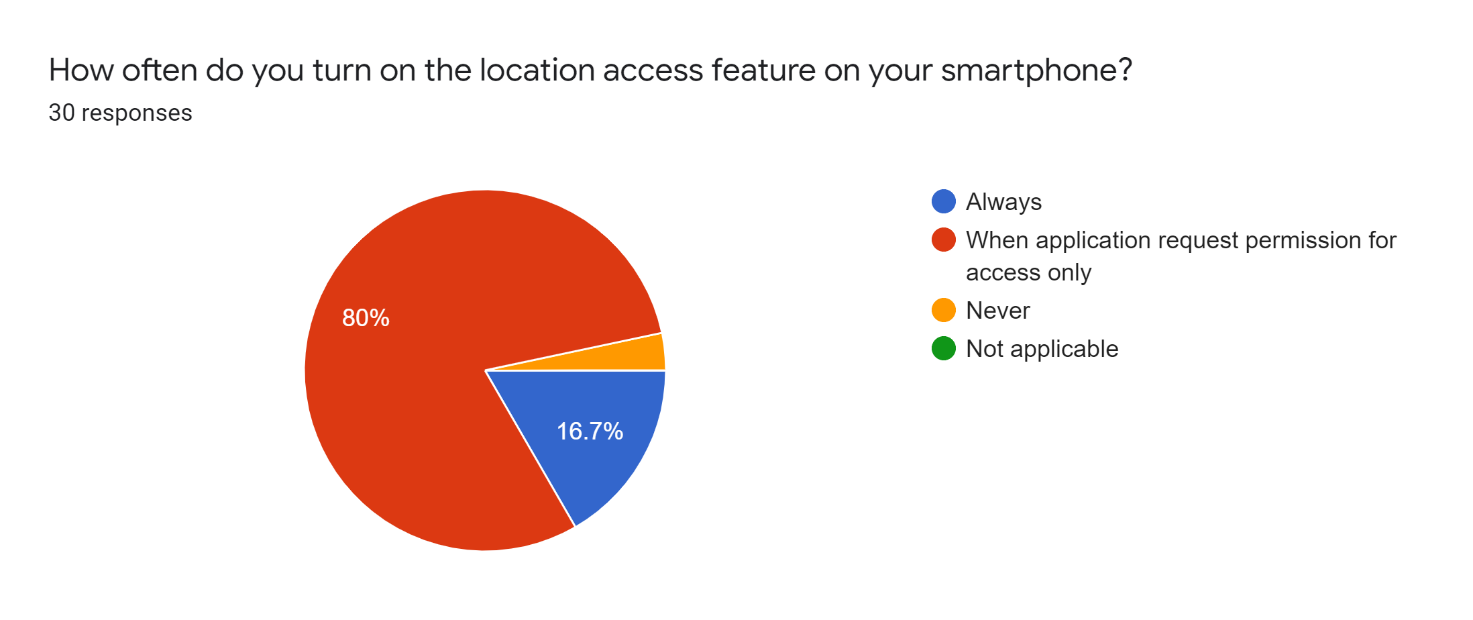
\includegraphics[width=18cm]{img/Survey/Q6.png}
      % \caption*{#3}
    \end{figure}
    \begin{figure}[H]
      \centering
      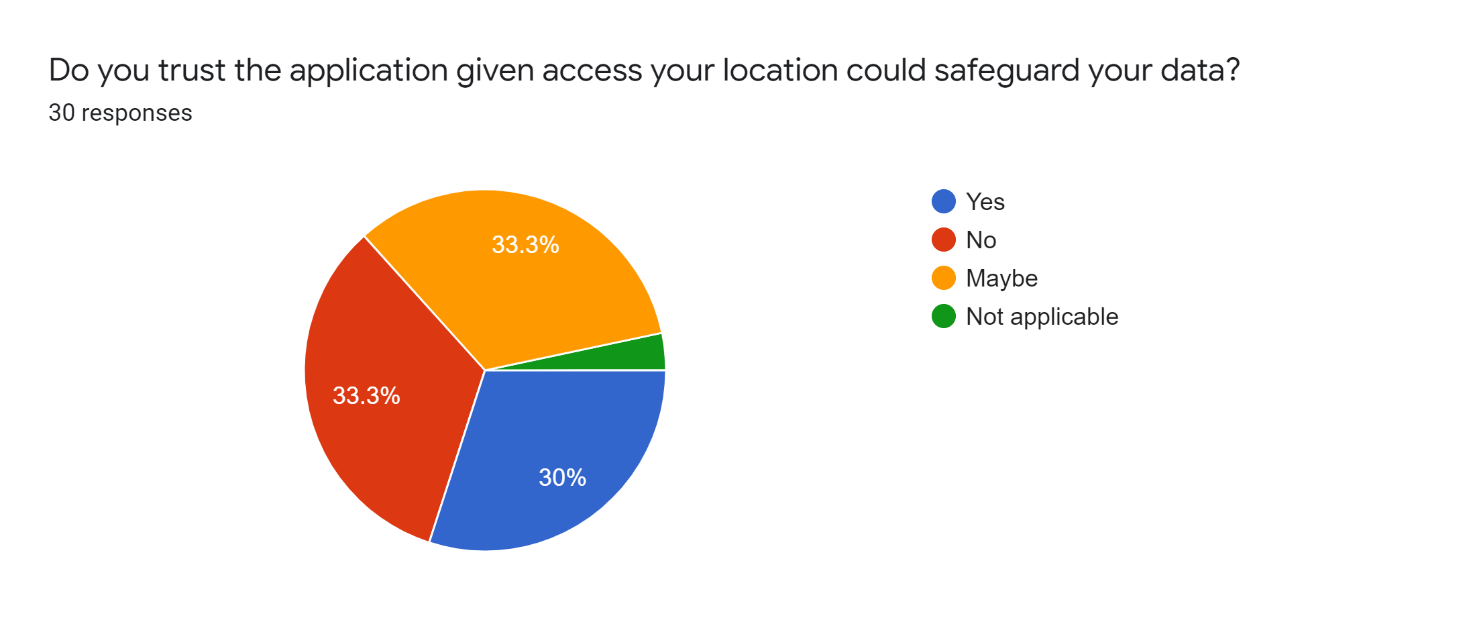
\includegraphics[width=18cm]{img/Survey/Q7.png}
      % \caption*{#3}
    \end{figure}
    \begin{figure}[H]
      \centering
      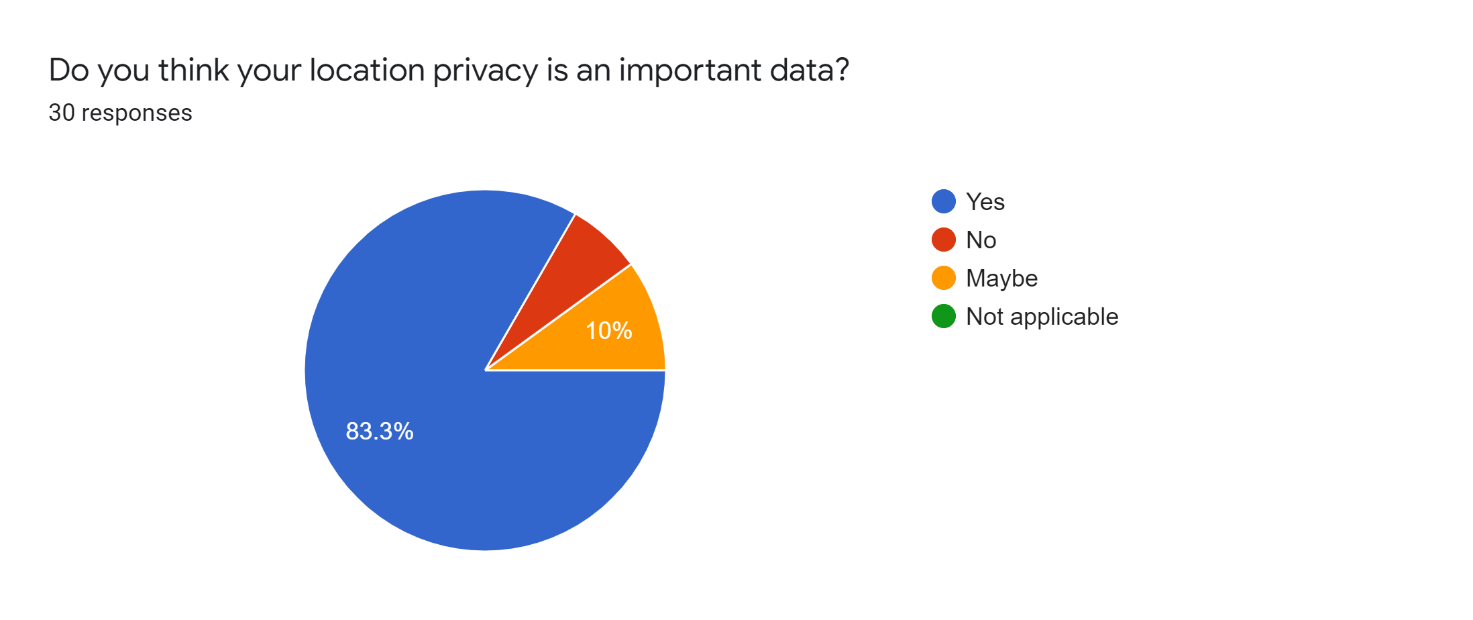
\includegraphics[width=18cm]{img/Survey/Q8.png}
      % \caption*{#3}
    \end{figure}
    \begin{figure}[H]
      \centering
      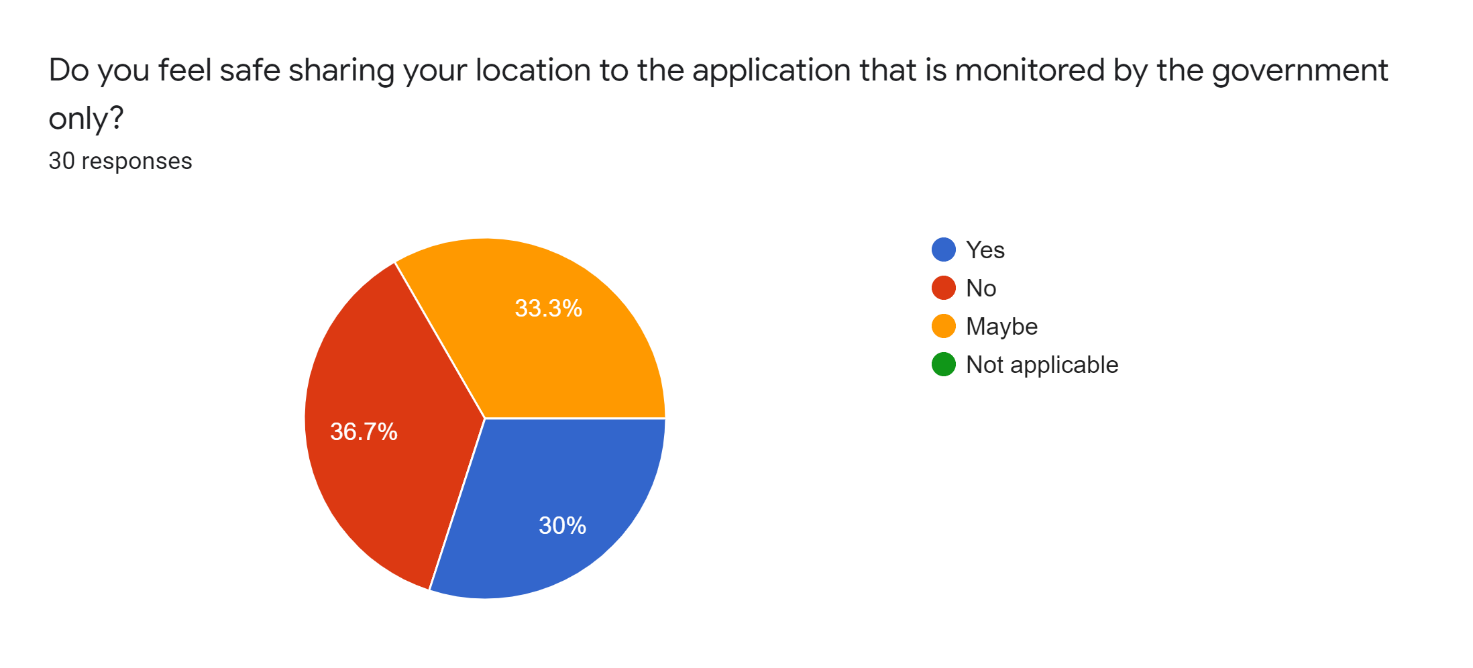
\includegraphics[width=18cm]{img/Survey/Q9.png}
      % \caption*{#3}
    \end{figure}

  \section{Qualitative Research - Interview} \label{appendix:qualitative}

    \subsection{Interview 1 Transcript (Primary School Student)}
      \begin{itemize}
        \item \textbf{Interviewer}: A
        \item \textbf{Interviewee \#1}: B
      \end{itemize}
      \par \textit{Answers are slightly modified for clarity purposes}

      \begin{itemize}
        \item A: Hi “B”, do you want your parents to accompany you during this session?
        \item B: Nope, I’m all good.
        \item A: OK, let’s start straight away.
        \item A: With the current pandemic situation in Australia, how do you find yourself coping with it?
        \item B: I am staying safe at home most of times. As my classes will be moved to a home-based
  learning on Term 2 onwards, my parents will want me to be a little more motivated in my
  studies. As I never done this before, I find myself a little scare especially not being able to
  play with my mates.
        \item A: Do you think the government is handling the current pandemic situation well?
        \item B: I’m not very sure how the government is responding to this situation, but I think some
  measures should be taken at an earlier stage when patients number are still low.
        \item A: Based on the data collection from my survey, around 60% of my respondents think that a
  pandemic tracking application is useful. What do you think?
        \item B: I think it would be more useful for my parents as they need to go outdoors for essential
  activities. As a kid of my age, I spent most of time at home like other of my mates as well. So,
  I think listening to my parents to stay at home would be safe enough without needing this
  application. My mates also told me that their parents do not allow them to join in groceries
  shopping as well. That is why I don’t think I need it since I’m listening to what my parents
  tell me. Also, I am not interested in knowing these things.
        \item A: Ok, let me end with one last question. Please tell me if you do not understand my question.
        \item B: Ok.
        \item A: Do you think your parents telling the government their real-time location through the
  smartphone is good or bad thing for safety purposes?
        \item B: As long as the government can keep my parents safe. If not, I think it is useless.
        \item A: What do you mean by that?
        \item B: I know from my mate that my parents sharing their location could also put me in risk as well
  if the data is not handled well, which I believe the government should be responsible for taking
  care my parents data, if not removing it.
        \item A: I think you are tired as well now. Thank you so much for your time. See you soon.
        \item B: Cheers.
      \end{itemize}

      \subsection{Interview 2 Transcript (Retail Worker)}
      \begin{itemize}
        \item \textbf{Interviewer}: A
        \item \textbf{Interviewee \#2}: C
      \end{itemize}
      \par \textit{Answers are slightly modified for clarity purposes}

      \begin{itemize}
        \item A: Morning “C”, are you prepared?
        \item C: Yes, let’s go.
        \item A: With the current pandemic situation in Australia, how do you find yourself coping with it?
        \item C: Well, I am currently rostered with a maximum of a 10 hours shift weekly, which I have been
        reduced to a quarter of my normal weekly shift hours. It’s kind of frustrating as I have
        mortgage and other commitments. I would say it is very tough for me during this period.
        \item A: Despite your reduced shift hours, I assume that you are still not thinking to stop temporarily
        with this ongoing pandemic situation?
        \item C: I would say it’s on a horn of a dilemma, I understand it’s between wealth or health, but I do
        not have a ticket for both sides, which is why I still choose to pay my bills.
        \item A: Besides that, do you think the government is handling the current pandemic situation well?
        \item C: I don’t think the government is enforcing enough restrictions on the movement control of the
        people. I believe it needs a more comprehensive strategy to monitor all the people that
        currently resides in Australia under this kind of situation.
        \item A: Following up on your response, how do you see a pandemic tracking application?
        \item C: It’s a good concept that can be made feasible. But I still have doubts with the government
        collecting my location data.
        \item A: So, what do you think can go wrong?
        \item C: I believed that our location data are considered personal information, which should be our
        user privacy as a fundamental rights. I think that the government needs a system that could
        prevent data breaches to allow the users feel safe giving consent to share this piece of
        information for all legal and valid purposes.
        \item A: For example, if a kind of security mechanism is used to safeguard the data, do you feel more
        confident in sharing the location data?
        \item C: I’m not tech savvy but I know there is no security system that is unbreachable now. I believe
        if the government could least create a top-tier security system, I would be joining as a user.
        \item A: I think that is all for me. I appreciate your valuable time and input for my further research.
        \item C: No worries, catch you later.
      \end{itemize}
  
    \subsection{Interview 3 Transcript (Retired Elderly)}
      \begin{itemize}
        \item \textbf{Interviewer}: A
        \item \textbf{Interviewee \#3}: D
      \end{itemize}
      \par \textit{Answers are slightly modified for clarity purposes}

      \begin{itemize}
        \item A: Hi “D”, how are you feeling today?
        \item D: Same as usual.
        \item A: So why not let us get this interview done and you could enjoy the rest of the day?
        \item D: I’ll be glad.
        \item A: Firstly, how do you find yourself coping with this current pandemic situation in Australia?
        \item D: I’m still alive and kicking but still very anxious when going out grabbing some essentials
        sometimes as you won’t know how well this fragile and vulnerable body could withstand.
        \item A: No worries “D”. I believe good hygienic practices could reduce the risk of being infected.
        Please don’t hesitate to contact me with any shopping if you need a helping hand.
        \item D: Nah, my kids would help me from time to time to stock up so no worries.
        \item A: Alright, so do you think the government is handling the current pandemic situation well?
        \item D: In terms on the restrictions and measures, there is still space for improvement to reduce the
        spread rate. As for caregiving support, I believe the government and other bodies have been
        doing well to support this community group of taking care of our wellbeing. My folks also
        told me that the government is close collaborating with NGO parties to prioritize medical
        support for our community. I am quite satisfied.
        \item A: How about the necessity of a pandemic tracking application then?
        \item D: I believed it would not be very convenient for an old folk like me and others. As I started
        experiencing functional loss on different aspects of my body following my days, I find
        difficulties in using digital devices other than calling someone now.
        \item A: I understand. If the application has a simple and friendly user interface, or even technology
        that assist disabilities. Do you think it will be more accepting in your community group?
        \item D: If additional support is provided in any form that could help us to understand the application.
        It would serve as a huge boost for older folks like us to use it. Count me in!
        \item A: Lastly, my research on a recent survey show that one-third of the respondents could trust the
        application with protecting the data, another one-third of not able to protect the data, and the
        remaining of having doubts with the application safeguarding the data respectively. So, what
        do you think about the data protection on an application?
        \item D: As much I am concerned with the data protection scheme of the application, I believe
        everything has a risk, nevertheless for this pandemic tracking application too. So, a method to
        earn the peoples’ trust is to formulate a best possible strategy that could mitigate to a minimum
        impact as much as possible.
        \item A: Thank you so much for your precious time and valuable input. Have a good day and take care.
        \item D: It’s my pleasure. See you.
      \end{itemize}

\end{appendices}

\newpage
\printbibliography

\end{document}
